\documentclass[a4paper,11pt,bibliography=totoc,listof=totoc,headinclude=true,cleardoublepage=empty,oneside]{scrbook}
% Option "oneside" für einseitigen Druck. Weglassen, falls die Arbeit doppelseitig gedruckt wird

\usepackage[english,ngerman]{babel}
\usepackage[utf8]{inputenc}
%\usepackage{fullpage}
\usepackage{ifthen}
\usepackage{color}
\usepackage{amsmath,amsthm,amssymb,amsfonts}
\usepackage{mathtools}
\usepackage{graphicx}
\usepackage{tikz}
\usetikzlibrary{calc}
\usepackage{psfrag}
\usepackage{algorithm}
\usepackage{algpseudocode}
\usepackage{float}

% links in pdf
\usepackage[unicode,colorlinks=true,pagebackref=false]{hyperref}

\newtheorem{theorem}{Theorem}[chapter]
\newtheorem{definition}[theorem]{Definition}
\newtheorem{cor}[theorem]{Corollary}
\newtheorem{rem}[theorem]{Remark}
\newtheorem{lemma}[theorem]{Lemma}
\newtheorem{prop}[theorem]{Proposition}

\newcommand{\R}{\mathbb{R}}
\newcommand{\N}{\mathbb{N}}
\newcommand{\Q}{\mathbb{Q}}
\newcommand{\Z}{\mathbb{Z}}
\renewcommand{\i}{\mathrm{i}}
\renewcommand{\Im}{\mathfrak{Im}}
\renewcommand{\Re}{\mathfrak{Re}}
\newcommand{\dff}{\Tilde{\beta}_\alpha}
\newcommand{\dffv}{\Tilde{\beta}_{\Vec{\alpha}}}
\newcommand{\bigO}{\mathcal{O}}
\newcommand{\F}{\mathcal{F}}
\newcommand{\e}{\mathrm{end}}

\algdef{SE}[DOWHILE]{Do}{doWhile}{\algorithmicdo}[1]{\algorithmicwhile\ #1}%


% Zum Druck verwende schwarze Links!
%\usepackage[unicode,colorlinks=true,linkcolor=black,citecolor=black,urlcolor=black,pagebackref=false]{hyperref} 
	% colorlinks=false umrahmt Links statt einzufaerben, 


% document style
\KOMAoptions{footinclude=false} % Fusszeile wird nicht zu Satzspiegel gezaehlt
\KOMAoptions{headsepline=true} % Trennlinie zwischen Kopfzeile und Text
\KOMAoptions{DIV=12} % beeinflusst Satzspiegel
\KOMAoptions{BCOR=8mm} % Bindekorrektur
\pagestyle{headings} % mit Kopfzeilen

\recalctypearea % berechne Satzspiegel neu

\definecolor{change}{rgb}{0,.55,.55}

\def\revision#1{{\color{red}#1}}


%%%%%%%%%%%%%%%%%%%%%%%%%%%%%%%%%%%%%%%%%%%%%%%%%%%%%%%%%%%%%%%%%%%%%%%%%%%%%%%%%%%%%%%%%%%%%%%%%%%%%%%%%%%%%%
%%%%%%%%%%%%%%%%%%%%%%%%%%%%%%%%%%%%%%%%%%%%%%%%%%%%%%%%%%%%%%%%%%%%%%%%%%%%%%%%%%%%%%%%%%%%%%%%%%%%%%%%%%%%%%
%%%%%%%%%%%%%%%%%%%%%%%%%%%%%%%%%%%%%%%%%%%%%%%%%%%%%%%%%%%%%%%%%%%%%%%%%%%%%%%%%%%%%%%%%%%%%%%%%%%%%%%%%%%%%%
%%%%%%%%%%%%%%%%%%%%%%%%%%%%%%%%%%%%%%%%%%%%%%%%%%%%%%%%%%%%%%%%%%%%%%%%%%%%%%%%%%%%%%%%%%%%%%%%%%%%%%%%%%%%%%

\begin{document}

%%%%%%%%%%%%%%%%%%%%%%%%%%%%%%%%%%%%%%%%%%%%%%%%%%%%%%%%%%%%%%%%%%%%%%%%%%%%%%%%%%%%%%%%%%%%%%%%%%%%%%%%%%%%%%
% TITELSEITE [OBLIGATORISCH]
%%%%%%%%%%%%%%%%%%%%%%%%%%%%%%%%%%%%%%%%%%%%%%%%%%%%%%%%%%%%%%%%%%%%%%%%%%%%%%%%%%%%%%%%%%%%%%%%%%%%%%%%%%%%%%

\pagenumbering{Alph}
\selectlanguage{ngerman}

\begin{titlepage}
  %\vspace*{-2cm}
  \begin{center}
    \includegraphics[width=0.45\textwidth]{TULogo.eps}
    \vskip 1cm%
    {\LARGE B~\Large A~C~H~E~L~O~R~A~R~B~E~I~T}
    \vskip 8mm
    {\huge\bfseries\color{change}Titel \\[1ex] ggf.\ mehrzeilig}
    \vskip 1cm
    \large 
    ausgef\"uhrt am    
    \vskip 0.75cm
    {\Large Institut f\"ur\\[1ex] Analysis und Scientific Computing}\\[1ex]
    {\Large TU Wien}
    \vskip0.75cm
    unter der Anleitung von
    \vskip0.75cm
    {\Large\bfseries 
Associate Prof. Dipl.-Math. Dr.rer.nat. Lothar Nannen \\ 
Univ.Ass. Dipl.-Ing. Dr.techn. Markus Wess}\\[1ex]
    \vskip 0.5cm
    durch
    \vskip 0.5cm
    {\Large\bfseries Michał Trojanowski}\\[1ex]
    Matrikelnummer: 12108865\\[1ex]
  \end{center}
  
  \vfill
  
  \small
  Wien, am \today
  \vspace*{-15mm}
\end{titlepage}

\cleardoublepage

%%%%%%%%%%%%%%%%%%%%%%%%%%%%%%%%%%%%%%%%%%%%%%%%%%%%%%%%%%%%%%%%%%%%%%%%%%%%%%%%%%%%%%%%%%%%%%%%%%%%%%%%%%%%%%
% DANKSAGUNG / ACKNOWLEDGEMENT [OPTIONAL]
%%%%%%%%%%%%%%%%%%%%%%%%%%%%%%%%%%%%%%%%%%%%%%%%%%%%%%%%%%%%%%%%%%%%%%%%%%%%%%%%%%%%%%%%%%%%%%%%%%%%%%%%%%%%%%

\chapter*{Danksagung} %\chapter*{Acknowledgement}
\thispagestyle{empty}
\selectlanguage{ngerman} %\selectlanguage{english}

{\color{change}
\begin{itemize}
\item auf Deutsch oder Englisch
\item Die Danksagung (engl. {\em Acknowledgement}) ist optional und kann auch entfallen. Denken Sie ggf.\ an Ihre eigenen Eltern!

\item Falls die Arbeit durch eine Forschungsprojekt finanziert wurde, so ist jedenfalls der Fördergeber (z.B.\ FWF oder WWTF) mit Projektnummer und Projektname zu nennen.
\begin{itemize}
\item siehe z.B.\ Dissertation von Michele Ruggeri:
\item[] \href{https://publik.tuwien.ac.at/files/publik_252806.pdf}{\ttfamily https://publik.tuwien.ac.at/files/publik\_252806.pdf}
\end{itemize}

\end{itemize}
}

\cleardoublepage

%%%%%%%%%%%%%%%%%%%%%%%%%%%%%%%%%%%%%%%%%%%%%%%%%%%%%%%%%%%%%%%%%%%%%%%%%%%%%%%%%%%%%%%%%%%%%%%%%%%%%%%%%%%%%%
% EIDESSTATTLICHE ERKLAERUNG [OBLIGATORISCH]
%%%%%%%%%%%%%%%%%%%%%%%%%%%%%%%%%%%%%%%%%%%%%%%%%%%%%%%%%%%%%%%%%%%%%%%%%%%%%%%%%%%%%%%%%%%%%%%%%%%%%%%%%%%%%%

\chapter*{Eidesstattliche Erkl\"arung}
\thispagestyle{empty}
\selectlanguage{ngerman}
\thispagestyle{empty}

\vspace*{2cm}

Ich erkl\"are an Eides statt, dass ich die vorliegende Bachelorarbeit selbstst\"andig und ohne fremde Hilfe verfasst, andere als die angegebenen Quellen und Hilfsmittel nicht benutzt bzw. die w\"ortlich oder sinngem\"a{\ss} entnommenen Stellen als solche kenntlich gemacht habe.

\vspace*{3cm}

\noindent
Wien, am \today
%
\hfill 
%
\begin{minipage}[t]{5cm}
\centering
\underline{\hspace*{5cm}}\\
\small{Michał Trojanowski}
\end{minipage}

\cleardoublepage

%%%%%%%%%%%%%%%%%%%%%%%%%%%%%%%%%%%%%%%%%%%%%%%%%%%%%%%%%%%%%%%%%%%%%%%%%%%%%%%%%%%%%%%%%%%%%%%%%%%%%%%%%%%%%%
% INHALTSVERZEICHNIS [OBLIGATORISCH]
%%%%%%%%%%%%%%%%%%%%%%%%%%%%%%%%%%%%%%%%%%%%%%%%%%%%%%%%%%%%%%%%%%%%%%%%%%%%%%%%%%%%%%%%%%%%%%%%%%%%%%%%%%%%%%

\pagenumbering{roman}
%\selectlanguage{ngerman} %
\selectlanguage{english} 

\tableofcontents

\cleardoublepage
\pagenumbering{arabic} 

%%%%%%%%%%%%%%%%%%%%%%%%%%%%%%%%%%%%%%%%%%%%%%%%%%%%%%%%%%%%%%%%%%%%%%%%%%%%%%%%%%%%%%%%%%%%%%%%%%%%%%%%%%%%%%
% EINLEITUNG / INTRODUCTION [OBLIGATORISCH]
%%%%%%%%%%%%%%%%%%%%%%%%%%%%%%%%%%%%%%%%%%%%%%%%%%%%%%%%%%%%%%%%%%%%%%%%%%%%%%%%%%%%%%%%%%%%%%%%%%%%%%%%%%%%%%

%%%%%%%%%%%%%%%%%%%%%%%%%%%%%%%%%%%%%%%%%%%%%%%%%%%%%%%%%%%%%%%%%%%%%%%%%%%%%%%%%%%%%%%%%%%%%%%%%%%%%%%%%%%%%%
%%%%%%%%%%%%%%%%%%%%%%%%%%%%%%%%%%%%%%%%%%%%%%%%%%%%%%%%%%%%%%%%%%%%%%%%%%%%%%%%%%%%%%%%%%%%%%%%%%%%%%%%%%%%%%
\chapter{Introduction}
\label{chapter:introduction}


\chapter{A Krylov eigenvalue solver based on filtered time domain solutions}
\label{chapter:ftd}
In this chapter, we present the concept of a Krylov eigenvalue solver for computing eigenvalues of the negative Laplace operator. By reformulating the problem to its weak form and selecting a finite solution space, we find that our problem is equivalent to a matrix eigenvalue problem for some high-dimensional matrix. The core idea of the Krylov eigenvalue solver is to construct a matrix $C$ that has the same eigenspaces as the original problem but different eigenvalues. Projection onto a lower-dimensional Krylov space generated by this matrix significantly reduces computational costs. We construct the operator $C$ by integrating in time a solution to the wave equation multiplied by some weight function. Proper selection of the weight function allows us to find eigenvalues of the original problem in the desired region. This chapter is based on \cite{nannen}.

\begin{definition}[Eigenvalue problem of the negative Laplace operator]\label{def:ev problem}
    Let $\Omega \subset \R^d$ for $d=2,3$ be a bounded domain with a Lipschitz boundary. We seek eigenvalues $\omega^2 \in \R_{+}$ and eigenfunctions $u\in H^1(\Omega)\backslash \{0\}$ of the negative Laplace operator with Neumann boundary conditions:
        \begin{align}\begin{split}\label{eq:ev problem}
              -\Delta u &= \omega^2 u \quad \text{ in } \Omega, \\
              \frac{\partial u}{\partial \nu} &= 0 \quad\text{ on } \partial\Omega.
        \end{split}\end{align}
    Here $\frac{\partial}{\partial\nu}$ denotes the normal derivative, and $H^1$ is the Sobolev space.
\end{definition}
Now we discretize the problem in space, fixing a partition $\mathcal{T}$ of $\Omega$. We introduce a discrete solution space as a finite-dimensional space of piecewise polynomials on $\Omega$.
\begin{definition}[Discrete solution space]\label{def:solution space}
Let $\mathcal{P}_p$ denote the space of polynomials up to degree $p \in \N$. We define the discrete solution space as
\begin{equation*}
V_h := \left\{v \in H^1(\Omega): \quad \forall T \in \mathcal{T}, \, v|_T \in \mathcal{P}_p \right\}
\end{equation*}
with finite dimension $N := \mathrm{dim} (V_h)$.
\end{definition}

Using Gauss's theorem, we can formulate both the weak and discrete forms of problem \eqref{eq:ev problem}.

\begin{definition}[Weak formulation of the eigenvalue problem]\label{def:weak form}
Let $\Omega$ be a bounded Lipschitz domain, as defined in Definition \ref{def:ev problem}, and $V_h$ be the discrete solution space. We seek eigenvalues $\omega_h^2 \in \R_+$ corresponding to discrete eigenfunctions $u \in V_h\backslash\{0\}$, such that for all test functions $\varphi \in V_h$, the following holds:
\begin{equation}\label{eq:weak form}
\int_\Omega \nabla u \cdot \nabla \varphi \, dx = \omega_h^2 \int_\Omega u \varphi \, dx.
\end{equation}
\end{definition}

To simplify notation in subsequent sections, we omit the index $h$ for discrete eigenfunctions and eigenvalues. We now demonstrate that the discrete eigenvalue problem \eqref{eq:weak form} reduces to a matrix eigenvalue problem, since the solution space is finite-dimensional.

\begin{definition}\label{def:SM matrices}
Let $V_h$ be an $N$-dimensional solution space with basis $(\varphi_1, \dots, \varphi_N)$. We define matrices $S:=(s_{ij})_{i, j=1}^N $ and $M:=(m_{ij})_{i, j=1}^N $ as follows:
\begin{equation*}
s_{ij} := \int_\Omega \nabla \varphi_i \cdot \nabla \varphi_j \, dx \quad \text{ and } \quad m_{ij} := \int_\Omega \varphi_i \varphi_j \, dx.
\end{equation*}
\end{definition}

\begin{lemma}
Equivalent to the problem stated in Definition \ref{def:weak form} is the eigenvalue problem to find non-trivial $v \in \R^N$ and $\omega^2 \in \R_+$ such that:
\begin{equation}\label{eq:matrix form}
Sv = \omega^2 Mv
\end{equation}
where $S, M \in \R^{N \times N}$ are defined in Definition \ref{def:SM matrices}.
\end{lemma}

\begin{proof}
Since $(\varphi_1, \dots, \varphi_N)$ forms a basis of $V_h$, it suffices, if \eqref{eq:weak form} holds for all basis functions. By representing $u$ with coordinate vector $v\in \R^N$, we can substitute $u = (\varphi_1, \dots, \varphi_N) v$. Thus, we obtain:
\begin{align*}
        \forall j=1, \dots, N : \, \int_\Omega (\nabla\varphi_1, \dots, \nabla\varphi_N)v\cdot \nabla \varphi_j \, dx &= \omega^2 \int_\Omega (\varphi_1, \dots, \varphi_N)v \varphi_j \, dx, \\
        \forall j=1, \dots, N : \, \int_\Omega (\nabla \varphi_j \cdot \nabla \varphi_1, \dots, \nabla \varphi_j \cdot \nabla \varphi_N) v \, dx &= \omega^2 \int_\Omega (\varphi_j\varphi_1, \dots, \varphi_j\varphi_N)v \,dx, \\ 
        \forall j = 1, \dots, N: \, (s_{j1},\dots,s_{jN})v &= \omega^2 (m_{j1},\dots, m_{jN})v,
\end{align*}
which is equivalent to \eqref{eq:matrix form}.
\end{proof}

\begin{rem}
Matrices $S$ and $M$ from Definition \ref{def:SM matrices} are self-adjoint. Furthermore, matrix $S$ is positive semi-definite and $M$ is positive-definite.
\end{rem}


\section{Elementary eigenvalue solvers for matrices}
Since we have approximated the eigenvalue problem of the negative Laplacian operator (see Definition \ref{def:ev problem}) into a matrix eigenvalue problem, we recall elementary numerical algorithms to solve such problems. For proofs of convergence of these algorithms, we refer to \cite{numericsAB}.

The first algorithm provides an approximation of an eigenvector corresponding to the eigenvalue with the largest absolute value among the eigenvalues of the matrix  under assumptions of Theorem \ref{theorem:power iteration}.

\begin{algorithm}[H]
\caption{Power iteration}\label{alg:power iteration}
\begin{algorithmic}
    \State \textbf{Input:} $A \in \R^{N \times N}$, start vector $v^{(0)}\in \R^N \backslash\{0\}$
    \For{$i = 1, 2, \dots$}
        \State $v \gets Av^{(i-1)} $
        \State $v^{(i)} \gets \frac{v}{\|v\|_2}$
    \EndFor
    \State \textbf{Output:} $v^{(i)}$ -- approximation of an eigenvector to the eigenvalue with the largest absolute value under assumptions of Theorem \ref{theorem:power iteration}.
    \end{algorithmic}
\end{algorithm}
\begin{theorem}\label{theorem:power iteration}
Let $A \in \R^{N \times N}$ be a diagonalizable matrix with eigenvalues $\mu_1, \dots, \mu_N$, such that $|\mu_1| > |\mu_2| \geqslant |\mu_j|$ for all $j = 3,\dots,N$. Let $(v_1, \dots, v_N)$ denote a basis of $\R^N$, such that for all $j=1, \dots N$, $v_j$ is a normed eigenvector to eigenvalue $\mu_j$. Let $v = \sum_{j=1}^N c_j v_j \in \R^N$ be a start vector, such that $c_1 \neq 0$. Then for all $i \in \N$, holds the error estimation for the eigenspace:
\begin{equation*}
        \left\| v^{(i)} - \frac{\mu_1^i c_1}{|\mu_1^i c_1|} v_1 \right\|_2 = \bigO\left( \left|\frac{\mu_2}{\mu_1}\right|^i\right) \text{ for } i \rightarrow \infty.
\end{equation*}
Furthermore, holds the error estimation for the convergence of the eigenvalue. Let $\mu^{(i)} := (Ax^{(i)})_k / x^{(i)}_k $ for some $k = 1, \dots, N$. It holds:
    \begin{equation*}
        |\mu_1 - \mu^{(i)}| = \bigO\left( \left|\frac{\mu_2}{\mu_1}\right|^i\right) \text{ for } i \rightarrow \infty.
    \end{equation*}
\end{theorem}
\begin{proof}
We refer to \cite[p. 116]{numericsAB}.
\end{proof}

The second algorithm enables us to compute the entire spectrum of a matrix under assumptions of Theorem \ref{theorem:QR alg}. 

\begin{algorithm}[H]
\caption{QR Algorithm}\label{alg:QR alg}
\begin{algorithmic}
    \State \textbf{Input:} $A \in \R^{N \times N}$
    \State $A^{(0)} \gets A$
    \For{$i = 1, 2, \dots$}
        \State compute QR-decomposition: $Q^{(i)} R^{(i)} = A^{(i-1)}$ 
        \State $A^{(i)} \gets R^{(i)}Q^{(i)}$
    \EndFor
    \State \textbf{Output:} $A^{(i)}$ -- approximation of an upper triangular matrix with eigenvalues of $A$ on the diagonal under assumptions of Theorem \ref{theorem:QR alg}. 
    \end{algorithmic}
\end{algorithm}

\begin{theorem}\label{theorem:QR alg}
    Let $A \in \R^{N \times N}$ be a diagonalizable matrix with pairwise different absolute values of eigenvalues: $\mu_1 > \mu_2 > \dots > \mu_N$. Let $\Lambda^{(i)} := \left(A^{(i)}_{11}, \dots, A^{(i)}_{NN}\right)$. Then $\Lambda^{(i)}$ converges linearly towards $(\mu_1, \dots, \mu_N)$ as $i\rightarrow\infty$. 
\end{theorem}

\begin{proof}
    We refer to \cite[p. 120]{numericsAB}.
\end{proof}

Since our goal is to find the eigenvalues of the negative Laplace operator, we could use the QR algorithm to obtain all eigenvalues of the discrete problem. However, this is not feasible due to the high computational costs of the QR algorithm. We focus on situations where the problem on the discrete level is high-dimensional. The QR algorithm demands the computation of a QR-decomposition of an $N \times N$ matrix in each iteration, which has cubic computational complexity. Therefore, this method is out of reach for our problem. We have to deploy a method that is based on a direct solver, such as the power iteration. 

\section{Krylov eigenvalue solver}

Now we need to make an assumption that there exists a matrix $C\in \R^{N \times N}$ such that its eigenvectors are linear combinations of eigenvectors of the discrete problem \eqref{eq:matrix form}. 

\begin{definition}\label{def:C}
    Let $C \in \R^{N\times N}$ be a matrix such that there exists an eigenvalue $\mu \in \R$ corresponding to the eigenvector $w\in \R^N$, i.e., $Cw = \mu w$, if and only if $w$ is an eigenvector or a linear combination of eigenvectors to some eigenvalue $\omega^2$ in the discrete problem \eqref{eq:matrix form}.
\end{definition}

We obtain properties of the matrix $C$ that will be needed. The exact choice and construction of this matrix will be discussed later. We recall the definition of a Krylov space.

\begin{definition}[Krylov space]
    Let $C \in \R^{N \times N}$ be a matrix and $r\in \R^N$ be a normalized start vector, i.e., $\|r\|_2=1$. For $m\in \N$, we define the Krylov space as a subspace of $\R^N$:
    \begin{equation*}
        \mathcal{K}_m(C; r) := \mathrm{span}\left\{r, Cr, \dots, C^{m-1}r\right\}.
    \end{equation*}
\end{definition}

In this thesis, we focus on situations where $N$ is large. Our goal is to project the $N$-dimensional eigenvalue problem \eqref{eq:matrix form} onto an $m$-dimensional Krylov space, using an orthonormal basis of this space. Typically, we choose $m$ much smaller than $N$, so that this problem is solvable with low computational costs using a direct solver.

Let $\mathcal{K}_m(C; r)$ be an $m$-dimensional Krylov space for matrix $C\in \R^{N\times N}$ and start vector $r\in \R^N$, where $\|r\|_2=1$. We obtain an orthonormal basis $(b_0, \dots, b_{m-1})$ of the Krylov space using Gram-Schmidt orthonormalization:
\begin{equation*}
    b_0 := r \quad \text{and} \quad \widetilde{b}_{j} := Cb_{j-1} - \sum_{i=0}^{j-1} (b_i^T C b_{j-1}) b_i, \quad b_j := \frac{\Tilde{b}_{j-1}}{\|\Tilde{b}_{j-1}\|_2} \quad \text{for all } j=1, \dots, m-1. 
\end{equation*}


Now we can project the original problem \eqref{eq:matrix form} onto the $m$-dimensional Krylov space.

\begin{prop}[Eigenvalue problem on Krylov space]
    Let $B_m = (b_0, \dots, b_{m-1}) \in \R^{N\times m}$ be an orthonormal basis of an $m$-dimensional Krylov space $\mathcal{K}_m(C; r)$. The eigenvalue problem on the Krylov space is to find eigenvalues $\omega_m^2 \in \R_+$ and eigenvectors $v_m\in\R^m$, such that:
    \begin{equation}\label{eq:Krylov problem}
        B_m^T S B_m v_m = \omega_m^2 B_m^T M B_m v_m.
    \end{equation}
\end{prop}
%TODO: proof????, Lemma? Theorem? 

Since matrices $S$ and $M$ are Hermitian, Krylov iteration leads to convergence of eigen-spaces of \eqref{eq:Krylov problem} towards the eigenspace of $C$ corresponding to the eigenvalue $\mu_{\max}$ with the largest absolute value. Obviously, projected eigenvalues $\omega_m^2$ converge towards the eigenvalue $\omega^2$ of the original problem \eqref{eq:matrix form} corresponding to $\mu_{\max}$.

To sum up the core idea of this section, we can explicitly formulate an (not yet implementable) algorithm based on Krylov spaces to compute eigenvalues $\omega^2$.

\begin{algorithm}[H]
\caption{Krylov eigenvalue solver}\label{alg:Krylov base}
    \begin{algorithmic}
        \State \textbf{Input:} matrix $C$, start vector $r$, $M^{-1}$, $S$, $m$ dimension of the Krylov space
        \State $b_0 \gets r$
        \For{$ k = 1, \dots, m-1$}
            \State $b_k \gets Cb_{k-1}$ \Comment{Krylov step}
            \State $b_{k} \gets b_k - \sum_{i=0}^{k-1} (b_i^T b_k) b_i$ \Comment{Gram-Schmidt orthogonalization}
            \State $ b_k \gets b_{k}/\|b_{k}\|_2 $\Comment{Normalization}
        \EndFor
        \State $B_m \gets (b_0, \dots, b_{m-1})$ \Comment{Projection matrix}
        \State $A \gets B_m^T M^{-1}S B_m$
        \State solve $Av = \omega_m^2 v$ with power iteration
    \end{algorithmic}
\end{algorithm}

Our goal is to compute eigenvalues $\omega^2$ of \eqref{eq:matrix form} in a given region of interest $\left[\omega_{\min}^2, \omega_{\max}^2\right]$. Therefore, we need matrix $C$ to fulfill the following four conditions.
\begin{itemize}
    \item $C$ satisfies the conditions in Definition \ref{def:C}.
    \item Eigenvalues $\mu$ corresponding to eigenspaces of eigenvalues $\omega^2$ in the region of interest have large absolute value.
    \item Eigenvalues $\mu$ corresponding to eigenspaces of eigenvalues $\omega^2$, which are not sought, are close to 0. 
    \item Each Krylov step $r \mapsto Cr$ can be computed with low cost.
\end{itemize}
In other words, the use of matrix $C$ filters sought eigenvalues from among all eigenvalues of the original problem \eqref{eq:matrix form} via common eigenspaces.

\begin{rem}
    Shift-and-inverse matrix:
    \begin{equation*}
        C_\rho := (S - \rho M)^{-1}M
    \end{equation*}
    for some $\rho \in \R$ has eigenvalue $\mu = (\omega^2 - \rho)^{-1}$ corresponding to the eigenspace to the eigenvalue $\omega^2$ of the original problem \eqref{eq:matrix form}. Therefore, $C_\rho$ with $\rho = (\omega^2_{\min}+\omega^2_{\max})/2 $ would be a possible choice of matrix $C$. Nevertheless, it requires the inverse of an $N\times N$ matrix $(S - \rho M)$, which for large $N$ is impossible with low computational complexity.
\end{rem}

\begin{proof}
    Let $(\mu, w)\in \R\times\R^N$ be an eigenpair of $C_\rho$. We note that $\mu \neq 0$, since matrices $(S-\rho M)^{-1}$ and $M$ have full rank. We have:
    \begin{align*}
        C_\rho w &= \mu w &&\iff \\
        (S - \rho M)^{-1}Mw &= \mu w  &&\iff \\
        \frac{1}{\mu}Mw &= (S - \rho M)w &&\iff \\
        Sw &= \underbrace{\left(\rho + \frac{1}{\mu}\right)}_{=\omega^2} Mw.&& 
    \end{align*}
    Therefore $\omega^2$ is an eigenvalue of $M^{-1}S$ to the eigenvector $w$. Conversely, if $\omega^2$ is an eigenvalue of $M^{-1}S$, then $\mu = (\omega^2 - \rho)^{-1}$ is an eigenvalue of $C_\rho$ to the same eigenvector. Obviously, $|\mu|$ takes on the largest values if $\omega^2 \approx \rho$.
\end{proof}

\section{Filtered time domain solutions}
To construct an appropriate finite-dimensional operator to replace the role of the matrix $C$ from the previous section, we proceed as follows. We consider the homogeneous wave equation with some initial condition $u_0 = (\varphi_1, \dots, \varphi_N)r$ projected onto our discrete solution space $V_h$ (see Definition \ref{def:solution space}). We discretize the problem in space and formulate its weak form. The evaluation of our operator $C$ at the point $r$ is a time-integral of the solution to this semi-discrete problem.

We consider the homogeneous 2- or 3-dimensional wave equation in $\Omega \times (0, \infty)$:
\begin{align}
\begin{split}\label{eq:wave equation}
    \ddot{u} = \Delta u \quad \text{in } \Omega \times (0, \infty), \quad  u = 0 \quad \text{in } \partial\Omega\times (0, \infty),\\
    u( \cdot, 0)= u_0, \quad \dot{u}(\cdot, 0) = 0 \quad \text{in } \Omega,
\end{split}
\end{align}
where $u$ is a function $\Omega \times [0, \infty) \rightarrow \R$ and $\ddot{u}$ denotes the second time-derivative.

\begin{prop}
    Let $V_h$ be a discrete solution space with basis $(\varphi_1, \dots, \varphi_N)$, and let $r$ denote the coordinate vector of the projection of $u_0$ onto $V_h$, i.e., $u_0 = (\varphi_1, \dots, \varphi_N)r$. Let $S$ and $M$ denote the matrices from Definition \ref{def:SM matrices}. Discretization in space of the problem \eqref{eq:wave equation} leads to the following linear system of ordinary differential equations:
    \begin{align}\label{eq:discr wave equation}
    \begin{split}
        M \ddot{y}(t; r) &= -S y (t; r) \quad \text{ for all } t \in (0, \infty) \\
        y(0; r) &= r, \quad \dot{y}(0; r) = 0. 
    \end{split}
    \end{align}
\end{prop}
\begin{proof}
    The theory of partial differential equations leads us to the ansatz $u(t, x) = \sum_{i=1}^\infty \kappa_i(t) \xi_i(x)$, where $\xi_i$ are the eigenfunctions of the negative Laplace operator \cite[p. 122]{Jungel}. Since we want to solve the problem in our solution space $V_h$, we can assume that $u(\cdot, t)=(\varphi_1, \dots, \varphi_N)y(t)$ for some vector-valued function $y: [0, \infty) \rightarrow \R^N$.

    We reformulate $\ddot{u} = \Delta u$ to its weak form:
    \begin{align*}
        \forall \varphi \in V_h : \, \int_\Omega \ddot{u} \varphi \, dx &= \int_\Omega \Delta u \varphi \, dx, \\
        \forall \varphi \in V_h : \, \int_\Omega \ddot{u} \varphi \, dx &= - \int_\Omega \nabla  u\cdot  \nabla \varphi \, dx.
    \end{align*}
    $V_h$ is a finite-dimensional space; therefore, the condition "for all test functions" is equivalent to the condition "for all basis test functions":
    \begin{align*}
        \forall j=1, \dots, N:\, \int_\Omega (\varphi_1, \dots, \varphi_N)\ddot{y} \varphi_j \, dx &= -  \int_\Omega (\nabla \varphi_1, \dots, \nabla \varphi_N)y\cdot  \nabla \varphi_j \, dx, \\
        M\ddot{y} &= -Sy.
    \end{align*}
    It remains to show the equivalence of initial conditions. For $u_0$, we have:
    \begin{equation*}
        (\varphi_1, \dots, \varphi_N)r = u_0 = u(\cdot, 0) = (\varphi_1, \dots, \varphi_N)y(0),
    \end{equation*}
    so $y(0) = r$ in $\Omega$, and similarly $\dot{y}(0) = 0$ in $\Omega$.
\end{proof}
Now we can solve the semi-discrete wave equation \eqref{eq:discr wave equation} to construct an integral operator. 
\begin{lemma}\label{lemma:y solution}
    The unique solution to \eqref{eq:discr wave equation} is:
    \begin{equation}\label{eq:solution wave eq}
        y(t; r) = \sum_{j=1}^N \cos(\omega_j t) (v_j^T r) v_j,
    \end{equation}
    where $(v_j)_{j=1}^N$ is an orthonormal basis of $\R^N$ of eigenvectors of matrix $M^{-1}S$ with corresponding eigenvalues $\omega_j^2$.
\end{lemma}
\begin{proof}
    Because of the symmetry of matrices $S$ and $M$, there exists an orthonormal basis $(v_j)_{j=1}^N$ of eigenvectors of $M^{-1}S$. We denote corresponding eigenvalues with $\omega_j^2$, $j=1, \dots N$. Obviously, for all $j=1, \dots, N$ and for all $c_{1j}, c_{2j}\in \R$, the function $t\mapsto \left(c_{1j} \cos(\omega_j t) + c_{2j} \sin(\omega_j t)\right)v_j$ solves the differential equation \eqref{eq:discr wave equation}. Due to the linearity of the problem, 
    \begin{equation*}
        y(t) = \sum_{j=1}^N \left(c_{1j} \cos(\omega_j t) + c_{2j} \sin(\omega_j t)\right)v_j
    \end{equation*}
    solves the differential equation. Initial values lead to the form \eqref{eq:solution wave eq}. The uniqueness of the solution follows from the Picard-Lindelöf theorem.
\end{proof}

Now we can define an integral operator that maps the initial value of the semi-discrete wave equation \eqref{eq:discr wave equation} to a weighted time-integral of its unique solution. The discrete form of this operator will take over the role of matrix $C$. Depending on the choice of the weight function, eigenvalues of this discrete operator may fulfill the requirements that we have set for matrix $C$ in the previous section. This will be discussed later in Chapter \ref{chapter:function}. 

\begin{definition}\label{def:pi_alpha}
    Let $\alpha: [0; \infty) \rightarrow \R$ be a piecewise continuous function with compact support. We define $\Pi_\alpha: \R^N \rightarrow \R^N$ as a linear operator:
    \begin{equation*}
        \Pi_\alpha r := \int_0^\infty \alpha(t) y(t;r) \,dt,
    \end{equation*}
    where $y(t;r)$ is the unique solution to \eqref{eq:discr wave equation} from Lemma \ref{lemma:y solution}.
\end{definition}

The following lemma determines the correspondence between eigenvalues of $\Pi_\alpha$ and eigenvalues of the original problem \eqref{eq:matrix form}.

\begin{lemma}
    Let $\beta_\alpha : [0, \infty) \rightarrow \R$ be a filter function defined by:
    \begin{equation}\label{eq:cont filter function}
        \beta_\alpha(\omega) := \int_0^\infty \alpha(t) \cos(\omega t) \,dt. 
    \end{equation}
    Then the following two statements hold.
    \begin{enumerate}
        \item If $\omega^2$ is an eigenvalue of \eqref{eq:matrix form} corresponding to eigenvector $v$, then $v$ is also an eigenvector of $\Pi_\alpha$ corresponding to eigenvalue $\beta_\alpha(\omega)$. 
        \item If $\lambda$ is an eigenvalue of $\Pi_\alpha$ to eigenvector $v$, then there exists an eigenvalue $\omega^2$ of \eqref{eq:discr wave equation} such that $\beta_\alpha (\omega) = \lambda$, and 
        \begin{equation*}
            v \in \bigoplus\{ U : \exists \omega \, U \text{ is eigenspace to eigenvalue to } \omega \text{ and } \beta_\alpha(\omega) = \lambda\}.
        \end{equation*}
    \end{enumerate}
\end{lemma}
\begin{proof}
    \begin{enumerate}
        \item Since $(v_j)_{j=1}^N$ is an orthonormal basis of eigenvectors of matrix $M^{-1}S$, every eigenvector of \eqref{eq:matrix form} equals $v_j$ from \eqref{eq:solution wave eq} for some $j=1, \dots, N$. Therefore $y(t, v) = \cos(\omega_j t)v$ and 
        \begin{equation*}
            \Pi_\alpha v = \int_0^\infty \alpha(t) \cos(\omega_j t) v \, dt = \beta_\alpha(\omega) v.
        \end{equation*}
        So the first claim holds.
        \item If $\lambda$ is an eigenvalue of $\Pi_\alpha$ with eigenvector $v$, then for all $k=1, \dots, N$ holds:
        \begin{align*}
             0 &= (\Pi_\alpha v - \lambda v)v_k = \int_0^\infty \alpha(t) \sum_{j=1}^N \cos(\omega_k t) (v_j^T v)\underbrace{(v_j^T v_k)}_{=\delta_{jk}} \, dt - \lambda v^Tv_k \\ &= \left(\int_0^\infty \alpha(t) \cos(\omega_kt) - \lambda \right)v_k^T v = (\beta_\alpha(\omega_k) - \lambda)v_k^T v.
        \end{align*}
        If $\beta_\alpha (\omega_k)\neq \lambda$, then $v_k^Tv = 0$. Therefore $v$ belongs to the sum of eigenspaces to eigenvalues such that $\beta_\alpha(\omega_k) = \lambda$. Moreover, $v$ is an eigenvector, so $v\neq 0$. Therefore, there exists at least one $k$ such that $v_k^T v \neq 0$, which implies $\beta_\alpha (\omega_k) = \lambda$. 
    \end{enumerate}
\end{proof}

\section{Time discretization}
In the previous section, we introduced an operator $\Pi_\alpha$ that could meet our eigenvalue requirements and replace the matrix $C$ in Krylov iteration. However, exact computation of the value $\Pi_\alpha r$ is impossible for two reasons: it demands an analytical solution $y(\cdot; r)$ to the semi-discrete wave equation \eqref{eq:discr wave equation} as well as the computation of an integral.

In numerical method, we replace the integral in the definition of $\Pi_\alpha$ by the rectangular rule. Since we only need the values of the function $y(\cdot; r)$ at quadrature nodes, we can discretize the problem \eqref{eq:discr wave equation} in time and compute an approximation of the exact solution at those points using the finite difference method.
\begin{lemma}[Finite difference method]\label{lemma:finite diffs}
    For a given function $y \in C^4 ([a, b])$ and a uniform mesh $(t_l := a+\tau l)_{l=0}^{L}$ with $L+1\in\N$ nodes and mesh-size $\tau = (a-b)/L$, for all $l=1, \dots, L-1$, we have:
    \begin{equation*}
        \ddot{y}(t_l) = \frac{y(t_{l+1}) - 2 y(t_l) + y(t_{l-1})}{\tau^2} + \bigO(\tau^2).
    \end{equation*}
\end{lemma}
\begin{proof}
    This follows from a straight-forward calculation using Taylor expansion of the function $y$. For details, see \cite[p. 93]{numodes}.
\end{proof}

\begin{prop}[Finite difference method for semi-discrete wave equation]
    Let $\tau>0$ be the step size of a uniform mesh on $[0, \infty)$. By replacing the second time derivatives in \eqref{eq:discr wave equation} with the finite differences from Lemma \ref{lemma:finite diffs}, we obtain the following approximation $y_l(r)$ of $y(\tau l; r)$ for all $l \in \N$:
    \begin{align}\label{eq:fd for wave eq}
    \begin{split}
        y_{l+1}(r) &:= -\tau^2M^{-1}S y_l(r) + 2y_l(r) - y_{l-1}(r) \quad \text{ for } l \in \N, \\
        y_0(r) &:= r, \quad y_1(r) := r - \frac{\tau^2}{2}M^{-1}Sr
    \end{split}
    \end{align}
\end{prop}
\begin{proof}
    For initial values, we have $y(0; r) = r = y_0(r)$. By Taylor expansion:
    \begin{equation*}
        y(\tau; r) = y(0; r) + \tau \dot{y}(0; r) + \frac{\tau^2}{2} \ddot{y}(0; r) + \bigO(\tau^3) .
    \end{equation*} 
    $y(\cdot; r)$ is a solution to \eqref{eq:discr wave equation}, thus $y(0; r) = r$, $\dot{y}(0; r) = 0$ and $\ddot{y}(0; r) = -M^{-1}Sy(0; r) = -M^{-1}Sr$. We get:
    \begin{equation*}
        y(\tau; r) = r - \frac{\tau^2}{2} M^{-1}Sr + \bigO(\tau^3) = y_{1}(r) + \bigO(\tau^3).
    \end{equation*}
    Replacing the second time derivative in \eqref{eq:discr wave equation} by finite difference leads to:
    \begin{align*}
        y(\tau(l+1); r) &- 2 y(\tau l; r) + y(\tau(l-1); r) = -\tau^2 M^{-1}S y(\tau l; r) + \bigO(\tau^4), \\
        y(\tau(l+1); r) &= -\tau^2 M^{-1}S y(\tau l; r) + 2y(\tau l; r) - y(\tau (l-1); r) + \bigO(\tau^4).
    \end{align*}
    Hence, $y_l(r)$ defined in \eqref{eq:fd for wave eq} approximates $y(\tau l; r)$ for all $l \in \N$.
\end{proof}

\begin{prop}[Discrete operator for Krylov iteration]\label{prop:C operator}
    Let $L \in \N$ be the number of quadrature nodes and $T>0$ be the upper bound of integration. Discretizing the operator $\Pi_\alpha$ (see Definition \ref{def:pi_alpha}) by the rectangular rule with step size $\tau = T/L$ and approximation $y(l\tau; r) \approx y_l(r)$ leads to the discrete operator $C : \R^N \rightarrow \R^N$:
    \begin{equation}\label{eq:C operator}
        r \mapsto Cr := \sum_{l=0}^{L-1} \tau \alpha(\tau l) y_l(r).
    \end{equation}
\end{prop}

The discrete operator $C$ defined in Proposition \ref{prop:C operator} allows us to avoid high computational costs in each Krylov step $r \mapsto Cr$. However, we have to verify the coincidence between eigenpairs of $C$ and eigenpairs of the original problem \eqref{eq:matrix form}. For this reason, we construct a discrete filter function as a discrete analogue of \eqref{eq:cont filter function}.

If $r$ is an eigenvector of the matrix $M^{-1}S$ with eigenvalue $\omega^2$, then the time-stepping \eqref{eq:fd for wave eq} takes the following form for all $n\in \N$:
\begin{equation}\label{eq:y_l q_l}
    y_l(r) = q_l(\omega)r  
\end{equation}
with $q_l(\omega)$ being the solution to the following recursion:
\begin{align}\label{eq:q def}
    \begin{split}
        q_{l+1}(\omega) &:= (2-\tau^2\omega^2) q_l(\omega) - q_{l-1}(\omega) \quad \text{ for } l \in \N,\\
        q_0(\omega) &:= 1, \quad q_1(\omega) := 1 - \frac{\tau^2\omega^2}{2} 
    \end{split}
\end{align}
This linear difference problem has unique solution, which will be needed later in Lemma \ref{lemma:dff}. Therefore, we analyze the behavior of the solution as $l$ tends to infinity.

\begin{lemma}[Courant--Friedrichs--Lewy condition for $q_l$]\label{lemma:cfl}
    For a given $\tau > 0$ and $\omega > 0$, the unique solution to \eqref{eq:q def} is:
    \begin{equation}\label{eq:q explicit}
        q_l(\omega) =  \frac{1}{2}\left( c(\omega)^l + \overline{c(\omega)}^l\right),
    \end{equation}
    where 
    \begin{equation*}
        c(\omega) := 1 - \frac{\tau^2 \omega^2}{2} + \i \sqrt{1 - \left(1 - \frac{\tau^2 \omega^2}{2}\right)^2}.
    \end{equation*}
    Therefore, if $\tau < 2/\omega$, then the CFL condition is satisfied and $|c(\omega)|=1$, implying the boundedness of $|q_l(\omega)|$ as $l \rightarrow \infty$. Otherwise, $|q_l(\omega)|$ is unbounded.
\end{lemma}
\begin{proof}
    The characteristic equation of the difference equation \eqref{eq:q def} is:
    \begin{equation*}
        c(\omega)^2 + (\tau^2\omega^2 - 2)c(\omega) + 1 = 0. 
    \end{equation*}
    If $\tau < 2/\omega$, then the solutions are:
    \begin{equation*}
        c(\omega) = 1 - \frac{\tau^2 \omega^2}{2} + \i \sqrt{1 - \left(1 - \frac{\tau^2 \omega^2}{2}\right)^2} \quad \text{ and } \quad \overline{c(\omega)} = 1 - \frac{\tau^2 \omega^2}{2} - \i \sqrt{1 - \left(1 - \frac{\tau^2 \omega^2}{2}\right)^2}.
    \end{equation*}
     Obviously, $|c(\omega)|=1$. Linearity of the recursion implies that the unique solution is given by $q_l(\omega) = C_1 c(\omega)^l + C_2 \overline{c(\omega)}^l$. From the initial values, we obtain a system of two equations for $C_1$ and $C_2$ with the solution $C_1 = C_2 = 1/2$.

    Therefore, representation \eqref{eq:q explicit} holds. If $\tau < 2/\omega$, then $\Re(c(\omega)) < 0$, and \eqref{eq:q explicit} remains bounded as $l\rightarrow \infty$. 
    
    Otherwise, if $\tau > 2/\omega$, then the roots of the characteristic equation are real:
    \begin{equation*}
        c(\omega) = 1 - \frac{\tau^2 \omega^2}{2} \pm \sqrt{\left(1 - \frac{\tau^2 \omega^2}{2}\right)^2 -1 }.
    \end{equation*}
    One of the roots is smaller than $-1$, so the solution to the linear difference equation cannot be bounded as $l\rightarrow\infty$.
\end{proof}

We recall the recursive definition of Chebyshev polynomials on the interval $[-1, 1]$ \cite[p. 23]{numericsAB} and observe connection between Chebyshev polynomials mapped to the interval $[0, 4/\tau^2]$ and $q_l(\omega)$.

\begin{definition}[Chebyshev polynomials]\label{def:chebyshev polynomials}
    For all $l\in \N$, the Chebyshev polynomials $T_l: [-1, 1] \rightarrow \R$ are defined as:
    \begin{equation*}
        T_0(x) := 1, \quad T_1(x) := x, \quad T_l(x) := 2xT_l(x) - T_{l-1}(x) \text{ for } l \geqslant 2.
    \end{equation*}
\end{definition}

\begin{lemma}\label{lemma:q chebyshev}
    Let $\tau > 0$. For $l\in \N$, let $\hat{T}_l : [0, 4/\tau^2] \rightarrow \R $ denote the $l$-th Chebyshev polynomial on $[0, 4/\tau^2]$, i.e., $\hat{T}_l := T_l \circ \Psi$ with affine mapping 
    \begin{equation*}
        \Psi: \begin{cases}\left[0, \frac{4}{\tau^2}\right] &\rightarrow [-1, 1]\\ x &\mapsto \frac{\tau^2 x}{2} - 1\end{cases}
    \end{equation*}
    and $T_l$ Chebyshev polynomials from Definition \ref{def:chebyshev polynomials}. Then for all $l\in \N$ and $q_l$ defined in \eqref{eq:q def} holds: 
    \begin{equation*}
        q_l(\omega) = (-1)^l \Hat{T_l}(\omega^2) \text{ for all } \omega \in \left[0, \frac{2}{\tau}\right].
    \end{equation*}
\end{lemma}
\begin{proof}
    From the definition of $\Hat{T_l}$ follows recursion:
    \begin{equation}\label{eq:recursion proof cheb}
        \Hat{T_0}(x) \equiv 1, \quad \Hat{T_1}(x) = \frac{\tau^2}{2}x - 1, \quad \Hat{T_l}(x) = 2\left(\frac{\tau^2}{2}x - 1\right)\Hat{T_l}(x) - \Hat{T}_{l-1}(x) \text{ for } l \geqslant 2.
    \end{equation}
    We prove the claim by induction. The case $l=0$ is trivial. For $l=1$, we have:
    \begin{equation*}
        \Hat{T}_1(\omega^2) = \frac{\tau^2\omega^2}{2} - 1 = -q_1(\omega).
    \end{equation*}
    In the induction step from \eqref{eq:recursion proof cheb} follows:
    \begin{align*}
        \Hat{T}_{l+1}(\omega^2) &= \left(\tau^2 \omega^2 -2\right) \Hat{T}_l(\omega^2) - T_{l-1}(\omega^2) \\ &= \left(\tau^2 \omega^2 -2\right) (-1)^l q_l(\omega) - (-1)^{l-1} q_{l-1}(\omega) \\ &= (-1)^{l+1} \left( \left(2-\tau^2\omega^2\right)q_l(\omega) - q_{l-1}(\omega)\right) = (-1)^{l+1} q_{l+1}(\omega).
    \end{align*}
    This concludes the proof.
\end{proof}

The matrix $M^{-1}S$ has spectral decomposition $M^{-1}S = V\mathrm{diag}(\omega_1^2, \dots, \omega_N^2)V^T$, thus there exists its square root $\sqrt{M^{-1}S} = V\mathrm{diag}(\omega_1, \dots, \omega_N)V^T$. 

\begin{lemma}\label{lemma:dff}
    Let $L\in \N$ be the number of quadrature nodes, $T$ be the upper bound of the integral, and $\tau = T/L$, as in Proposition \ref{prop:C operator}. Let $q_l(\omega)$ be defined for all $l \in \N$ and $\omega \in \R$ by \eqref{eq:q def}. We define the discrete filter function $\dff: [0, \infty) \rightarrow \R$ as follows:
    \begin{equation}\label{eq:dff}
        \dff(\omega) := \sum_{l=0}^{L-1} \tau \alpha(\tau l) q_l(\omega).
    \end{equation}
    \begin{enumerate}
        \item $\dff$ is a polynomial of degree $L-1$ in $\omega^2$.
        \item For $C$ defined in Proposition \ref{prop:C operator}, $C = \dff\left(\sqrt{M^{-1}S}\right)$.
        \item If $(\omega^2, v)$ is an eigenpair of the original problem \eqref{eq:matrix form}, then $(\dff(\omega), v)$ is an eigenpair of $C$.
        \item If $(\lambda, v)$ is an eigenpair of $C$, then there exists $\omega \in \R$ such that $\omega^2$ is an eigenvalue of \eqref{eq:matrix form}, $\dff(\omega)=\lambda$, and
        \begin{equation*}
            v \in \bigoplus\{ U : \exists \omega \, U \text{ is eigenspace to eigenvalue } \omega \text{ and } \dff(\omega) = \lambda\}.
        \end{equation*}
    \end{enumerate}
\end{lemma}
\begin{proof}
    The first claim follows directly from the construction of $q_l(\omega)$ \eqref{eq:q def}. Let $V: = (v_1, \dots, v_N)$ be an orthonormal basis of eigenvectors corresponding to eigenvalues $\omega_1^2, \dots, \omega_N^2$ of $M^{-1}S$. The spectral decomposition of $M^{-1}S$ is $M^{-1}S = V \mathrm{diag}(\omega_1^2, \dots, \omega_N^2) V^T$. Since \eqref{eq:fd for wave eq} is a linear difference equation, for arbitrary $r\in\R^N$ and for all $l\in \N$ we obtain:
    \begin{equation*}
        y_l(r) = y_l \left( \sum_{j=1}^N (r^T v_j)v_j \right) = \sum_{j=1}^N (r^T v_j)y_l(v_j) \stackrel{\eqref{eq:y_l q_l}}{=} \sum_{j=1}^N (r^T v_j)q_l(\omega_j)v_j.
    \end{equation*}
    Therefore, by the definition of $C$:
    \begin{align*}
        Cr &= \sum_{l=0}^{L-1} \tau\alpha(l\tau) y_l(r) = \sum_{j=1}^N \sum_{l=0}^{L-1} \tau\alpha(l\tau)q_l(\omega_j) (r^T v_j) v_j \\ &= \sum_{j=1}^{N}\dff(\omega_j)(r^Tv_j)v_j = V \mathrm{diag}\left(\dff(\omega_1), \dots, \dff(\omega_N)\right)V^Tr = \dff\left(\sqrt{M^{-1} S}\right)r.
    \end{align*}
    So the second statement holds. The third and fourth claims follow from the second one. Let $\dff(\omega) = \sum_{l=0}^{L-1} c_l \omega^{2l}$ for some $c_0, \dots, c_{L-1}\in \R$. If $v$ is an eigenvector of \eqref{eq:matrix form} to eigenvalue $\omega^2$, then:
    \begin{equation*}
        Cv = \dff\left(\sqrt{M^{-1}S}\right)v = \sum_{l=0}^{L-1} c_l (M^{-1}S)^{l}v = \sum_{l=0}^{L-1} c_l \omega^{2l}v = \dff(\omega)v,
    \end{equation*}
    so $\dff(\omega)$ is an eigenvalue of $C$ to $v$. If $(\lambda, v)$ is an eigenpair of $C$, then for all $k=0,\dots, N$ holds:
    \begin{align*}
        0 &= (Cv - \lambda v)v_k = \left(\left(\dff\left(\sqrt{M^{-1}S}\right)v_k\right)^Tv - \lambda v^T v_k\right) \\&= \dff(\omega_k)v_k^T v - \lambda v^T v_k = \left(\dff(\omega_k) - \lambda\right)v^T v_k.
    \end{align*}
    Since $v^Tv_k \neq 0$ for some $k=1, \dots, N$, it follows that $\lambda = \dff(\omega_k)$ and $v$ belongs to the sum of all eigenspaces corresponding to eigenvalues $\omega^2$, such that $\dff(\omega) = \lambda$.
\end{proof}

\section{Algorithm}
Now that we have constructed the operator $C$ meeting our requirements, we can reformulate Algorithm \ref{alg:Krylov base} into an implementable form.

\begin{algorithm}[H]
\caption{Krylov eigenvalue solver with filtered time-domain}\label{alg:Krylov pro}
   \begin{algorithmic}
        \State \textbf{Input: } weight function $\alpha$, start vector $r$ with $\|r\|_2 = 1$, $M^{-1}$, $S$, dimension $m$ of the Krylov space, time-step $\tau$, number of time-steps $L$
        \State $b_0 \gets r$
        \For{$k = 1, \dots, m-1$}\Comment{Krylov loop}
            \State $y_{0} \gets b_{k-1}$, $y_1 \gets b_{k-1} - \frac{\tau^2}{2}M^{-1}Sb_{k-1}$
            \State $b_k \gets \tau \alpha(0) y_0 + \tau\alpha(\tau)y_1$ \Comment{First two summands in \eqref{eq:C operator}}
            \For{$l = 2, \dots L-1$}\Comment{Time-stepping in each Krylov step}
                \State $y_l \gets -\tau^2 M^{-1}S y_{l-1} + 2y_{l-1} - y_{l-2}$ \Comment{$y_l$ represents $y_l(r)$ from \eqref{eq:fd for wave eq}}
                \State $b_k \gets b_k + \tau \alpha(\tau l)y_l$ \Comment{Computation of $b_{k-1}\mapsto b_k := Cb_{k-1}$}
            \EndFor
            \State $b_k \gets b_k - \sum_{i=0}^{k-1}(b_i^Tb_k)b_i$ \Comment{Gram-Schmidt orthogonalization}
            \If{$\|b_k\|_2 \neq 0$}
                \State $b_k\gets b_k/\|b_k\|_2$ \Comment{Normalization}
            \Else
            \State $m\gets k$   \Comment{$b_k \in \mathrm{span}\{b_0, \dots, b_{k-1}\}$. Exact eigenspace is a subspace of $\mathcal{K}_k(C; r)$.}
                \State \textbf{break} 
            \EndIf
        \EndFor
        \State $B_m \gets (b_0, \dots, b_{m-1})$ \Comment{Projection matrix}
        \State $A \gets B_m^T M^{-1}S B_m$
        \State solve $Av_m = \omega_m^2 v_m$ with power iteration
    \end{algorithmic} 
\end{algorithm}

The chosen time-step $\tau$ should fulfill the CFL condition (see Lemma \ref{lemma:cfl}) for the largest absolute value among the eigenvalues $\omega^2$ of \eqref{eq:matrix form}. The computational complexity of this method depends on the number of time-steps $L$ (and thus by the end time of integration $T = \tau L$) and the dimension of the Krylov space $m$. Notice that in the presented algorithm, we can easily increase the dimension of the Krylov space without incurring significantly higher computational costs, since increasing $m$ by $\hat{m}$ requires only $\hat{m}$ additional iterations of the Krylov loop and solving the eigenvalue problem with power iteration. For more details about the stopping criterion, we refer to \cite[p. 8--9]{nannen}. In the next chapter, we will discuss the choice of the weight function $\alpha$.



\chapter{Choice of the weight function}
\label{chapter:function}
To fully enable the functionality of the Krylov eigenvalue solver based on filtered time-domain, we need an appropriate weight function $\alpha$. The first section of this chapter follows the choice in \cite{nannen}. In subsequent sections, we discuss other numerical methods for selecting the weight function.

The entire spectrum of eigenvalues $\omega^2$ of the discrete approximation \eqref{eq:matrix form} of the negative Laplacian eigenvalue problem is included within some interval $\left[0, \omega_\e^2\right]$. We search for eigenvalues within a specified region of interest $\left[\omega_{\min}^2, \omega_{\max}^2\right] \subset \left[0, \omega_\e^2\right]$. By employing the Krylov eigenvalue solver (Algorithm \ref{alg:Krylov pro}), we can compute eigenvalues $\omega^2$ such that the absolute value of the discrete filter function $\left|\dff(\omega)\right|$ is maximized.

Consequently, our goal is to construct a weight function $\alpha$ such that the filter function $\left|\beta_\alpha\right|$ \eqref{eq:cont filter function} or its discrete equivalent $\left|\dff\right|$ \eqref{eq:dff} takes on larger values if $\omega \in \left[\omega_{\min}, \omega_{\max} \right]$ and is close to 0 otherwise. Of course, we can require this only in the controlled interval $\left[0, \omega_\e\right]$, since, according to Lemma \ref{lemma:dff}, $\dff$ is a polynomial. Moreover, we require that the function $\alpha$ is piecewise continuous and compactly supported (see Definition \ref{def:pi_alpha}).

\section{Inverse Fourier transform method}
In this section, we follow the choice in \cite{nannen}. The first presented method of selecting a weight function is based on the observation that the mapping $\alpha \mapsto \beta_\alpha$ is somehow similar to the Fourier transform.
\begin{lemma}\label{lemma:alpha fourier}
    Let $\alpha$ be a piecewise continuous weight function with compact support and $\alpha \in L^1\left( [0, \infty) \right)$. Let $\hat{\alpha}: \R \rightarrow \R$ denote its symmetric extension, i.e., $\hat{\alpha}(-t) := \alpha(t)$ for all $t\in \R_+$. Then, for all $s\in \R$:
    \begin{equation*}
        \beta_\alpha (s) = \sqrt{\frac{\pi}{2}} \F\left[\hat{\alpha}\right] (s),
    \end{equation*}
    where $\mathcal{F}$ denotes the Fourier transform and $\beta_\alpha$ denotes the filter function  defined in \eqref{eq:cont filter function}.
\end{lemma}
\begin{proof}
    Obviously, if $\alpha \in L^1\left([0, \infty)\right)$, then $\hat{\alpha} \in L^1\left(\R\right)$. From \eqref{eq:cont filter function}, it follows:
    \begin{align*}
        \beta_\alpha (s) &= \int_0^\infty \alpha(t) \cos(s t) \,dt = \frac{1}{2}\int_{-\infty}^\infty \hat{\alpha}(t) \cos(s t) \,dt + \frac{\i}{2} \underbrace{\int_{-\infty}^\infty \hat{\alpha}(t) \sin(-st) \,dt}_{=0} \\&= \frac{1}{2} \int_{-\infty}^{\infty} \hat{\alpha}(t) e^{-\i st} \, dt = \sqrt{\frac{\pi}{2}} \F\left[\hat{\alpha}\right] (s).
    \end{align*}
    The sine-integral is 0, since $\hat{\alpha}$ is an even function and $t \mapsto \sin(-st)$ is an odd function. This proves the desired identity.
\end{proof}

This motivates the choice of the function $\alpha$ as the truncated inverse Fourier transform. As the goal function to be the filter function $\beta_\alpha$, we choose the symmetrical indicator function of the region of interest: $\chi_{\left[-\omega_{\max}, -\omega_{\min}\right]\cup\left[\omega_{\min}, \omega_{\max}\right]}$. Thanks to the symmetry of this function, its inverse Fourier transform is real-valued.

\begin{theorem}
    Truncation of the scaled inverse Fourier transform of the symmetric indicator function $\chi_{\left[-\omega_{\max}, -\omega_{\min}\right]\cup\left[\omega_{\min}, \omega_{\max}\right]}$ to a compact interval $[0, T]$, $T>0$, leads to the following weight function:
    \begin{equation}\label{eq:alpha fourier}
        \alpha(t) = \begin{cases}
            \frac{2\left(\omega_{\max} - \omega_{\min}\right)}{\pi}, \quad & t = 0, \\
            \frac{4}{\pi t} \sin\left(\frac{t}{2}\left(\omega_{\max}-\omega_{\min} \right)\right)\cos\left(\frac{t}{2}\left(\omega_{\max}+\omega_{\min} \right)\right), \quad & t \in (0, T], \\
            0, \quad & \text{else.}
        \end{cases}
    \end{equation}
\end{theorem}
\begin{proof}
    Following Lemma \ref{lemma:alpha fourier}, we compute:
    \begin{align*}
        \sqrt{\frac{2}{\pi}} \F^{-1}\left[\chi_{\left[-\omega_{\max}, -\omega_{\min}\right]\cup\left[\omega_{\min}, \omega_{\max}\right]}\right](t) &= \frac{1}{\pi} \int_{-\infty}^\infty \chi_{\left[\omega_{\min}, \omega_{\max}\right]} e^{\i st} \, ds \\ 
        & = \frac{1}{\pi} \left( \int_{-\omega_{\max}}^{-\omega_{\min}} \cos(st) \, ds + \int_{\omega_{\min}}^{\omega_{\max}} \cos(st) \, ds\right) \\ &+ \frac{\i}{\pi} \underbrace{\left(\int_{-\omega_{\max}}^{-\omega_{\min}} \sin(st) \, ds + \int_{\omega_{\min}}^{\omega_{\max}} \sin(st) \, ds \right)}_{=0} \\
        &= \frac{2}{\pi}\int_{\omega_{\min}}^{\omega_{\max}} \cos(st) \, ds \\
        &= \frac{2}{\pi t} \left(\sin\left(t\omega_{\max}\right) - \sin\left(t\omega_{\min}\right)\right) \\
        &= \frac{4}{\pi t} \sin\left(\frac{t}{2}\left(\omega_{\max}-\omega_{\min} \right)\right)\cos\left(\frac{t}{2}\left(\omega_{\max}+\omega_{\min} \right)\right).
    \end{align*}
    The obtained function is real-valued, but does not have compact support. Therefore, we truncate it to the finite interval $(0, T]$ and set $\alpha|_{(T, \infty)} := 0$. Since the limit from the right as $t\rightarrow 0^+$ is finite, we can right-continuously in 0 extend the function to the interval $[0, \infty)$. This leads to representation \eqref{eq:alpha fourier}.
\end{proof}

Since the discretization \eqref{eq:dff} of the filter function $\beta_\alpha$ truncates the time-interval, we truncate the weight function $\alpha$ to the same time $T>0$ as assumed in $\dff$. Of course, replacing the exact improper integral in the definition of $\beta_\alpha$ \eqref{eq:cont filter function} by a quadrature rule on a finite time-interval impacts the function, and therefore, the discrete filter function $\dff$ cannot be exactly the target indicator function $\chi_{\left[\omega_{\min}, \omega_{\max}\right]}$. However, for our purposes, it is sufficient if $\dff$ takes on larger values in the region of interest $\left[\omega_{\min}, \omega_{\max}\right]$ and is close to 0 otherwise.

The computational costs of the Krylov eigenvalue solver depend on the number of time-steps $L=T/\tau$. The CFL condition (see Lemma \ref{lemma:cfl}) allows us to choose time-step at most as $\tau = 2/\omega_{\e}$.

We choose the setup in \cite[section 3.1.2]{nannen}: $\tau = 0.0056$, $\omega_\e = 2/\tau \approx 357.14$, and varying end-times $T$ and target intervals $\left[\omega_{\min}, \omega_{\max}\right]$. Results are presented in Figures \ref{fig:fourier1} and \ref{fig:fourier2}. In each figure, the first plot presents the whole controlled interval $\left[0, \omega_\e\right]$, and the second plot shows the behavior of the discrete filter function in the region of interest compared to the target indicator function.

We can observe that for small values of $L$, the discrete filter function $\dff$ at the end of the controlled interval (for $\omega \approx \omega_\e$) may exceed its values in the target interval, which is unacceptable. Numerical experiments showed that increasing the number of time steps $L$ (and thus increasing the degree of the polynomial $\dff$) causes better behavior in both the target interval and the neighborhood of $\omega_\e$ and solves this issue. However, increasing $L$ is undesirable since it increases the computational costs of the algorithm.

It's worth noticing that the presented method can be extended for target functions other than the indicator. An arbitrary target function $\gamma$ on the interval $[0, \infty)$ can be symmetrically extended to the whole real domain. This always yields a real-valued inverse Fourier transform. Truncation of this function to the interval $[0, T]$ fulfills the requirements set on the weight function.

\begin{figure}[h]
    % left margin: 54 pt
    % top/bottom margin: 24 pt
    % first 50: 47 pt
    
    \centering
    \begin{tikzpicture}
        \node[inner sep=0pt] (image1) at (0,0) {\includegraphics[width=\textwidth]{latex//images//fourier/Figure_1.png}};
        
        \pgfmathsetmacro{\imagewidth}{\textwidth}
        \pgfmathsetmacro{\imageheight}{\textwidth / \pgfkeysvalueof{/pgf/outer xsep} * \pgfkeysvalueof{/pgf/outer ysep}}
    
        \pgfmathsetmacro{\xoffset}{0.002\textwidth}
        \node[anchor=center, inner sep=0pt] (image2) at ($ (image1.center) - (\xoffset, 0) $) {\includegraphics[width=0.4\textwidth]{latex//images//fourier/Figure_2.png}};
    
        % Draw a frame around the second image
        \draw[black] (image2.north west) rectangle (image2.south east);
    
        % rectangle in main image
        \draw[black] ($(image1.north west) + (54pt, -24pt)$) rectangle ($(image1.south west) + (73pt, 24pt)$);
    
        \draw [dashed] ($(image1.north west) + (73pt, -24pt)$) -- (image2.north west);
        \draw [dashed] ($(image1.south west) + (73pt, 24pt)$) -- (image2.south west);
    
        
    \end{tikzpicture}
    \caption{Plots of the function $\left|\dff(\omega) \right|$ with the weight function $\alpha$ obtained by truncated inverse Fourier transform \eqref{eq:alpha fourier}. The target interval is $\left[\omega_{\min}, \omega_{\max} \right] = [3, 6]$, the time-step is $\tau = 0.0056$, and $\omega_\e = 2/\tau \approx 357.14$. We vary the number of time-steps $L$.}
    \label{fig:fourier1}
\end{figure}

\begin{figure}[h]
    % left margin: 54 pt
    % top/bottom margin: 24 pt
    % first 50: 47 pt
    
    \centering
    \begin{tikzpicture}
        \node[inner sep=0pt] (image1) at (0,0) {\includegraphics[width=\textwidth]{latex//images//fourier/Figure_4.png}};
        
        \pgfmathsetmacro{\imagewidth}{\textwidth}
        \pgfmathsetmacro{\imageheight}{\textwidth / \pgfkeysvalueof{/pgf/outer xsep} * \pgfkeysvalueof{/pgf/outer ysep}}
    
        \pgfmathsetmacro{\xoffset}{0.002\textwidth}
        \node[anchor=center, inner sep=0pt] (image2) at ($ (image1.center) - (\xoffset, 0) $) {\includegraphics[width=0.4\textwidth]{latex//images//fourier/Figure_5.png}};
    
        % Draw a frame around the second image
        \draw[black] (image2.north west) rectangle (image2.south east);
    
        % rectangle in main image
        \draw[black] ($(image1.north west) + (54pt, -24pt)$) rectangle ($(image1.south west) + (73pt, 24pt)$);
    
        \draw [dashed] ($(image1.north west) + (73pt, -24pt)$) -- (image2.north west);
        \draw [dashed] ($(image1.south west) + (73pt, 24pt)$) -- (image2.south west);
    
        
    \end{tikzpicture}
    \caption{Plots of the function $\left|\dff(\omega) \right|$ with the weight function $\alpha$ obtained by truncated inverse Fourier transform \eqref{eq:alpha fourier}. The target interval is $\left[\omega_{\min}, \omega_{\max} \right] = [12, 14]$, the time-step is $\tau = 0.0056$, and $\omega_\e = 2/\tau \approx 357.14$. We vary the number of time-steps $L$.}
    \label{fig:fourier2}
\end{figure}

% TODO: Positioning of these figures
%\begin{figure}
%    \centering
%    \includegraphics[width=1\linewidth]{latex//images//fourier/Figure_1.png}
%    \includegraphics[width=1\linewidth]{latex//images//fourier/Figure_2.png}
%    \caption{Plots of the function $\left|\dff(\omega) \right|$ with the weight function $\alpha$ obtained by truncated inverse Fourier transform \eqref{eq:alpha fourier}. The target interval is $\left[\omega_{\min}, \omega_{\max} \right] = [3, 6]$, the time-step is $\tau = 0.0056$, and $\omega_\e = 2/\tau \approx 357.14$. We vary the number of time-steps $L$.}
%    \label{fig:fourier1}
%\end{figure}
%\begin{figure}
%    \centering
%    \includegraphics[width=1\linewidth]{latex//images//fourier/Figure_4.png}
%    \includegraphics[width=1\linewidth]{latex//images//fourier/Figure_5.png}
%    \caption{Plots of the function $\left|\dff(\omega) \right|$ with the weight function $\alpha$ obtained by truncated inverse Fourier transform \eqref{eq:alpha fourier}. The target interval is $\left[\omega_{\min}, \omega_{\max} \right] = [12, 14]$, the time-step is $\tau = 0.0056$, and $\omega_\e = 2/\tau \approx 357.14$. We vary the number of time-steps $L$.}
%    \label{fig:fourier2}
%\end{figure}

\section{Collocation method}\label{section:collocation}
The definitions of the discrete operator $C$ for Krylov iteration \eqref{eq:C operator} and of the discrete filter function $\dff$ \eqref{eq:dff} for a fixed time-step $\tau$ and number of time-steps $L$ do not require the values of the weight function in the whole domain, but only at $\tau l$ for $l=0, \dots, L-1$. Thus, we can reduce the problem to finding a vector $\Vec{\alpha} \in \R^L$, such that $\Vec{\alpha}_l$ represents the value $\alpha(\tau l)$ for all $l=0, \dots, L-1$.

\begin{definition}\label{def:dffv}
    Let $\tau > 0$ be the time-step, $L\in \N$ be the number of time-steps and let $q_l(\omega)$ be defined for all $l \in \N$ and $\omega \in \R$ by \eqref{eq:q def}. Let $\Vec{\alpha}\in\R^L$ be a weight vector. Then, the discrete filter function $\dffv: [0, \infty) \rightarrow \R$ is defined as:
    \begin{equation}\label{eq:dffv}
        \dffv (\omega) := \tau \left(q_0(\omega), \dots, q_{L-1}(\omega)\right) \Vec{\alpha}. 
    \end{equation}
\end{definition}

Note that for a given weight function $\alpha: \left[0, \omega_\e\right] \rightarrow \R$ and a vector $\Vec{\alpha} = \left(\alpha(\tau l)\right)_{l=0}^{L-1}$, the definition of $\dff$ in Lemma \ref{lemma:dff} is equivalent to Definition \ref{def:dffv}, i.e., $\dff = \dffv$.

We fix an arbitrary target function $\gamma$ that fulfills our requirements for the discrete filter function in the controlled interval. We select $L$ nodes in the controlled interval, in the simplest setting equidistant, and formulate our problem as a polynomial collocation problem with $\left\{q_l : l=0, \dots, L-1\right\}$ basis of the space of polynomials up to degree $L-1$ in $\omega^2$.
\begin{definition}\label{def:evaluation matrix}
    For given number of time-steps $L\in \N$ and $K\in \N$ collocation nodes $ 0 \leqslant \omega_0 < \dots < \omega_{K-1} \leqslant \omega_\e$ we define the evaluation matrix $Q \in \R^{K\times L}$ as $Q_{kl} := q_l\left(\omega_k\right)$ for all $k=0, \dots, K-1$ and $l=0, \dots, L-1$. 
\end{definition}

Let $\tau>0$ be the time-step, $L\in \N$ be the number of time-steps and $\left[\omega_{\min}, \omega_{\max}\right]$ denote the target interval. Selecting $L$ equidistant collocation nodes $\omega_l = l\omega_\e/ (L-1)$, $l=0, \dots, L-1$, in the controlled interval $\left[0, \omega_{\e}\right]$ leads to collocation problem to find $\Vec{\alpha} \in \R^L$, such that:
\begin{equation*}
    \forall k = 0, \dots, L-1: \quad \dffv\left(\omega_k\right) = \gamma(\omega_k).
\end{equation*}
This problem is equivalent to the linear system of equations:
\begin{equation}\label{eq:alpha eq coll}
     Q \Vec{\alpha} = \frac{1}{\tau} \left(\gamma(\omega_k) \right)_{k=0}^{L-1}
\end{equation}
with matrix $Q$ from Definition \ref{def:evaluation matrix}.

As an example, we choose the same parameters as in the previous section, especially the target function as an indicator of the target interval $\gamma = \chi_{\left[\omega_{\min}, \omega_{\max}\right]}$. Plots of the obtained discrete filter functions for two values of $L = 10 $ and $L=25$ are shown in Figure \ref{fig:eq coll beta}. We solve the system of linear equations \eqref{eq:alpha eq coll} with the \texttt{numpy.linalg.solve()} function in Python.

\begin{figure}[h]
    \centering
    \includegraphics[width=1\linewidth]{latex//images//equi_coll/Figure_1.png}
    \caption{Plots of the function $\left|\dffv\right|$ with $\Vec{\alpha}$ obtained by collocation \eqref{eq:alpha eq coll}. The target interval is $\left[\omega_{\min}, \omega_{\max} \right] = [39, 45]$, the time-step is $\tau = 0.0056$, and $\omega_\e = 2/\tau \approx 357.14$. We vary the number of time-steps and collocation nodes $L$. Crosses represent the values of the target function at the knots.}
    \label{fig:eq coll beta}
\end{figure}

By a small number of collocation knots, intervals between nodes are large, and we can observe strong oscillation of the polynomial, especially for larger values of $\omega$. Increasing the number of nodes does not improve the behavior for two reasons. Firstly, this increases the degree of the polynomial, which compounds the problem despite shorter intervals between nodes. Secondly, higher values of $L$ rapidly worsen the conditioning of the matrix $Q$. Figure \ref{fig:eq coll cond} presents $\mathrm{cond}(Q) := \|Q\|_2 \|Q^{-1}\|_2$ (where $\| \cdot \|_2$ denotes the induced matrix norm by the Euclidean norm) depending on the size of the problem $L$.

\begin{figure}
    \centering
    \includegraphics[width=1\linewidth]{latex//images//equi_coll/Figure_2.png}
    \caption{The condition number of the evaluation matrix $Q$ (matrix norm induced by the Euclidean norm) depending on the number of collocation nodes $L$.}
    \label{fig:eq coll cond}
\end{figure}

Because equidistant nodes in the collocation method do not produce desired results, we attempt to replace them. From Lemma \ref{lemma:q chebyshev}, we know that functions $q_l(\omega)$ are polynomials in $\omega^2$. The next proposition shows that the natural choice is Chebyshev collocation in $\omega^2$.

\begin{prop}[Chebyshev nodes] \label{def:chebyshev nodes}
    For $L\in\N$, Chebyshev nodes on the interval $(-1, 1)$ are given by:
    \begin{equation*}
        t_l := \cos\left(\frac{2l+1}{2L}\pi\right) \text{ for } l = 0, \dots, L-1.
    \end{equation*}
    \begin{enumerate}
        \item The Chebyshev polynomial $T_L$ (see Definition \ref{def:chebyshev polynomials}) has $L$ roots in the interval $(-1, 1)$, which are exactly the Chebyshev nodes.
        \item For $f \in C^{L}\left([a,b]\right)$, arbitrary collocation nodes $x_0, \dots, x_{L-1} \in [a,b]$ and Lagrange collocation polynomial $p\in \mathcal{P}_{L-1}$ such that $p(x_l) = f(x_l)$ for all $l=0, \dots, L-1$, there holds the error estimation:
        \begin{equation}\label{eq:lagrange error est}
            \|f-p\|_\infty \leqslant \frac{\|f^{(L+1)}\|_\infty}{(L+1)!} \max_{x\in[a,b]} \prod_{l=0}^{L-1} \left|x-x_l\right|.
        \end{equation}
        \item The affine transformation $\Psi: [-1, 1] \rightarrow [a,b]$, $\Psi(x) := \left(a+b+x(b-a)\right)/2$ maps Chebyshev nodes $t_0, \dots, t_{L-1}$ onto $\Psi(t_0), \dots, \Psi(t_{L-1}) \in [a,b]$. These nodes minimize the product in the error estimation, i.e.,
        \begin{equation*}
            \min_{(x_0, \dots, x_{L-1})\in [a,b]^L}  \max_{x\in[a,b]} \prod_{l=0}^{L-1} \left|x-x_l\right| =  \max_{x\in[a,b]} \prod_{l=0}^{L-1} \left|x-\Psi(t_l)\right| = \left(\frac{b-a}{2}\right)^{L} 2^{1-L}.
        \end{equation*}
    \end{enumerate}
\end{prop}
\begin{proof}
    We refer to \cite[p. 23--24]{numericsAB}.
\end{proof}

For a fixed time-step $\tau>0$, we choose collocation nodes $\omega_0, \dots, \omega_{L-1} \in \left[0, 2/\tau\right]$, such that $\omega_0^2, \dots, \omega_{L-1}^2$ are Chebyshev nodes in the interval $\left[0, 4/\tau^2\right]$, and solve the linear system of equations \eqref{eq:alpha eq coll}. Figures \ref{fig:cheb coll 1} and \ref{fig:cheb coll 2} show the obtained discrete filter functions $\left|\dffv\right|$ for different numbers of time-steps $L$ and target intervals $\left[\omega_{\min}, \omega_{\max} \right]$. We compare the behavior of the obtained discrete filter function with the target function and the inverse Fourier transformation \eqref{eq:alpha fourier} method.


\begin{figure}[h]
    % left margin: 54 pt
    % top/bottom margin: 24 pt
    % first 50: 47 pt
    
    \centering
    \begin{tikzpicture}
        \node[inner sep=0pt] (image1) at (0,0) {\includegraphics[width=\textwidth]{latex//images//cheb_coll/Figure_1.png}};
        
        \pgfmathsetmacro{\imagewidth}{\textwidth}
        \pgfmathsetmacro{\imageheight}{\textwidth / \pgfkeysvalueof{/pgf/outer xsep} * \pgfkeysvalueof{/pgf/outer ysep}}
    
        \pgfmathsetmacro{\xoffset}{0.002\textwidth}
        \node[anchor=center, inner sep=0pt] (image2) at ($ (image1.center) - (\xoffset, 0) $) {\includegraphics[width=0.4\textwidth]{latex//images//cheb_coll/Figure_2.png}};
    
        % Draw a frame around the second image
        \draw[black] (image2.north west) rectangle (image2.south east);
    
        % rectangle in main image
        \draw[black] ($(image1.north west) + (54pt, -24pt)$) rectangle ($(image1.south west) + (77.5pt, 24pt)$);
    
        \draw [dashed] ($(image1.north west) + (77.5pt, -24pt)$) -- (image2.north west);
        \draw [dashed] ($(image1.south west) + (77.5pt, 24pt)$) -- (image2.south west);
    \end{tikzpicture}
    \caption{Plots of the function $\left|\dffv\right|$ with $\Vec{\alpha}$ obtained by collocation with Chebyshev nodes in $\omega^2$. The target interval is $\left[\omega_{\min}, \omega_{\max} \right] = [12, 14]$, with a time-step of $\tau = 0.0056$ and $\omega_\e = 2/\tau \approx 357.14$. We vary the number of time-steps and collocation nodes $L$. Crosses represent values of the target function at the knots. The yellow curve represents the discrete filter function obtained by the inverse Fourier transform of the indicator truncated to end-time $T=2.8$.}
    \label{fig:cheb coll 1}
\end{figure}

%\begin{figure}
%    \centering
%    \includegraphics[width=1\linewidth]{latex//images//cheb_coll/Figure_1.png}
%    \includegraphics[width=1\linewidth]{latex//images//cheb_coll/Figure_2.png}
%    \caption{Plots of the function $\left|\dffv\right|$ with $\Vec{\alpha}$ obtained by collocation with Chebyshev nodes in $\omega^2$. The target interval is $\left[\omega_{\min}, \omega_{\max} \right] = [12, 14]$, with a time-step of $\tau = 0.0056$ and $\omega_\e = 2/\tau \approx 357.14$. We vary the number of time-steps and collocation nodes $L$. Crosses represent values of the target function at the knots. The yellow curve represents the discrete filter function obtained by the inverse Fourier transform of the indicator truncated to end-time $T=2.8$.}
%    \label{fig:cheb coll 1}
%\end{figure}

\begin{figure}[h]
    % left margin: 54 pt
    % top/bottom margin: 24 pt
    % first 50: 47 pt
    
    \centering
    \begin{tikzpicture}
        \node[inner sep=0pt] (image1) at (0,0) {\includegraphics[width=\textwidth]{latex//images//cheb_coll/Figure_3.png}};
        
        \pgfmathsetmacro{\imagewidth}{\textwidth}
        \pgfmathsetmacro{\imageheight}{\textwidth / \pgfkeysvalueof{/pgf/outer xsep} * \pgfkeysvalueof{/pgf/outer ysep}}
    
        \pgfmathsetmacro{\xoffset}{0.002\textwidth}
        \node[anchor=center, inner sep=0pt] (image2) at ($ (image1.center) + (110pt, -60pt) $) {\includegraphics[width=0.45\textwidth]{latex//images//cheb_coll/Figure_4.png}};
    
        % Draw a frame around the second image
        \draw[black] (image2.north west) rectangle (image2.south east);
    
        % rectangle in main image
        \draw[black] ($(image1.north west) + (157.4pt, -24pt)$) rectangle ($(image1.south west) + (195pt, 24pt)$);
    
        \draw [dashed] ($(image1.north west) + (195pt, -24pt)$) -- (image2.north west);
        \draw [dashed] ($(image1.south west) + (195pt, 24pt)$) -- (image2.south west);
    \end{tikzpicture}
    \caption{Plots of the function $\left|\dffv\right|$ with $\Vec{\alpha}$ obtained by collocation with Chebyshev nodes in $\omega^2$. The target interval is $\left[\omega_{\min}, \omega_{\max} \right] = [122, 130]$, with a time-step of $\tau = 0.0056$ and $\omega_\e = 2/\tau \approx 357.14$. We vary the number of time-steps and collocation nodes $L$. Crosses represent values of the target function at the knots. The yellow curve represents the discrete filter function obtained by the inverse Fourier transform of the indicator truncated to end-time $T=2.8$.}
    \label{fig:cheb coll 2}
\end{figure}

%\begin{figure}
%    \centering
%    \includegraphics[width=1\linewidth]{latex//images//cheb_coll/Figure_3.png}
%    \includegraphics[width=1\linewidth]{latex//images//cheb_coll/Figure_4.png}
%    \caption{Plots of the function $\left|\dffv\right|$ with $\Vec{\alpha}$ obtained by collocation with Chebyshev nodes in $\omega^2$. The target interval is $\left[\omega_{\min}, \omega_{\max} \right] = [122, 130]$, with a time-step of $\tau = 0.0056$ and $\omega_\e = 2/\tau \approx 357.14$. We vary the number of time-steps and collocation nodes $L$. Crosses represent values of the target function at the knots. The yellow curve represents the discrete filter function obtained by the inverse Fourier transform of the indicator truncated to end-time $T=2.8$.}
%    \label{fig:cheb coll 2}
%\end{figure}

Error estimation for Lagrange interpolation \eqref{eq:lagrange error est}, which was our motivation to replace equidistant nodes with Chebyshev ones, demands a function $\gamma$ that is $L$-times continuously differentiable, which is not the case for the indicator function. Therefore, in the third example, we change our target function to a $C^\infty$ function, the Gaussian peak $g(\omega) = \exp\left(-(\omega-\omega_{\mathrm{mid}})^2\right)$ with $\omega_{\mathrm{mid}}$ in the middle of the region of interest. Results are presented in Figure \ref{fig:cheb coll cont ex}. Again, we compare the obtained discrete filter function to one produced with the truncated inverse Fourier transform in a similar way to the derivation of \eqref{eq:alpha fourier}.

A remarkable advantage of collocation in Chebyshev nodes is the good conditioning of the collocation matrix $Q$. The condition number for Chebyshev nodes is, in contrast to equidistant nodes, independent of the size of the problem $L$. Furthermore, the obtained discrete filter function does not oscillate strongly between collocation knots, even for an uncontinuous target function like the indicator.

Following \cite{nannen}, we assume that the sought eigenvalues of the negative Laplace operator are closer to 0 than to the end of the controlled interval $\omega_\e$. Chebyshev nodes in $\omega^2$ have the highest density in the upper area of the interval $[0, \omega_\e]$. Thus, especially for lower numbers of collocation knots and a small target interval, the entire interval $\left[\omega_{\min}, \omega_{\max} \right]$ may be contained between two consecutive nodes. This sets the right-hand side of the collocation problem \eqref{eq:alpha eq coll} to 0, and as a result, we get $\Vec{\alpha}=0$ and $\dffv \equiv 0$. We can observe this problem in Figure \ref{fig:cheb coll 1} for $L=100$. In this particular example, $ 8.4142\approx\omega_1 < \omega_{\min} = 12 < 14 = \omega_{\max} < \omega_2 \approx 14.0213 $. Also, a small shift of the target interval does not impact the discrete filter function at all if the change in $\omega_{\min}$ and $\omega_{\max}$ does not exceed the distance to the nearest nodes. A similar problem can be observed for the $C^\infty$ target function for $L=100$ in Figure \ref{fig:cheb coll cont ex}.

Obviously, with increasing $L$, the distances between nodes decrease, which solves this issue. However, this is undesired, since we want to choose $L$ as small as possible due to the complexity of the Algorithm. Another possibility would be to increase the number of collocation nodes $K$ by the same number of basis functions $L$. This would lead to a $K\times L$ evaluation matrix with $K>L$ and a least squares problem instead of a linear system of equations.

\begin{figure}[h]
    % left margin: 54 pt
    % top/bottom margin: 24 pt
    % first 50: 47 pt
    
    \centering
    \begin{tikzpicture}
        \node[inner sep=0pt] (image1) at (0,0) {\includegraphics[width=\textwidth]{latex//images//cheb_coll/Figure_5.png}};
        
        \pgfmathsetmacro{\imagewidth}{\textwidth}
        \pgfmathsetmacro{\imageheight}{\textwidth / \pgfkeysvalueof{/pgf/outer xsep} * \pgfkeysvalueof{/pgf/outer ysep}}
    
        \pgfmathsetmacro{\xoffset}{0.002\textwidth}
        \node[anchor=center, inner sep=0pt] (image2) at ($ (image1.center) - (\xoffset, 0) $) {\includegraphics[width=0.4\textwidth]{latex//images//cheb_coll/Figure_6.png}};
    
        % Draw a frame around the second image
        \draw[black] (image2.north west) rectangle (image2.south east);
    
        % rectangle in main image
        \draw[black] ($(image1.north west) + (54pt, -24pt)$) rectangle ($(image1.south west) + (77.5pt, 24pt)$);
    
        \draw [dashed] ($(image1.north west) + (77.5pt, -24pt)$) -- (image2.north west);
        \draw [dashed] ($(image1.south west) + (77.5pt, 24pt)$) -- (image2.south west);
    \end{tikzpicture}
    \caption{Plots of the function $\left|\dffv\right|$ with $\Vec{\alpha}$ obtained by collocation in Chebyshev nodes in $\omega^2$. The target function is $g(\omega) = \exp\left(-(\omega-4)^2\right)$, with a time-step of $\tau = 0.0056$ and $\omega_\e = 2/\tau \approx 357.14$. We vary the number of time-steps and collocation nodes $L$. Crosses represent values of the target function at the knots. The yellow curve represents the discrete filter function obtained by the inverse Fourier transform of the indicator truncated to end-time $T=2.8$.}
    \label{fig:cheb coll cont ex}
\end{figure}

%\begin{figure}
%    \centering
%    \includegraphics[width=1\linewidth]{latex//images//cheb_coll/Figure_5.png}
%    \includegraphics[width=1\linewidth]{latex//images//cheb_coll/Figure_6.png}
%    \caption{Plots of the function $\left|\dffv\right|$ with $\Vec{\alpha}$ obtained by collocation in Chebyshev nodes in $\omega^2$. The target function is $g(\omega) = \exp\left(-(\omega-4)^2\right)$, with a time-step of $\tau = 0.0056$ and $\omega_\e = 2/\tau \approx 357.14$. We vary the number of time-steps and collocation nodes $L$. Crosses represent values of the target function at the knots. The yellow curve represents the discrete filter function obtained by the inverse Fourier transform of the indicator truncated to end-time $T=2.8$.}
%    \label{fig:cheb coll cont ex}
%\end{figure}

\section{Least squares method and minimization of $L^2$ norm}
We start this section with the idea of fixing the number $L$ of time-steps (and thus the polynomial degree) to avoid increasing the computational costs of the algorithm, while simultaneously increasing the number of collocation knots. Obviously, the obtained system of equations is (in general) not solvable, so we use linear least squares fitting. Then we switch to another approach -- we try to find $\Vec{\alpha}$ that minimizes the $L^2$ norm of the difference between the corresponding discrete filter function and the target function $\gamma$. Finally, Theorem \ref{theorem:lsq converges to l2} will show the connection between these two methods.

\begin{definition}[Least squares method]\label{def:least sq}
    Let $\tau>0$ denote the time-step and $L \in \N$ denote the number of time-steps. For given nodes $\omega_0, \dots, \omega_{K-1} \in [0, \omega_\e]$ with $K>L$, let $Q\in\R^{K\times L}$ denote the evaluation matrix from Definition \ref{def:evaluation matrix}. For a piecewise continuous target function $\gamma : [0, \omega_\e] \rightarrow \R$, we search for $\Vec{\alpha} \in \R^{L}$, such that:
    \begin{equation}\label{eq:least sq}
        \| Q\vec{\alpha} - c \|_2 = \min_{x\in \R^L} \| Qx - c \|_2,
    \end{equation}
    where $c := 1/\tau \left(\gamma(\omega_0), \dots, \gamma(\omega_{K-1})\right)^T$.
\end{definition}

Note that the problem stated in Definition \ref{def:least sq} is just a modification of the collocation problem \eqref{eq:alpha eq coll} for the case $K>L$.

\begin{prop}[Normal equation]\label{prop:normal eq}
    The problem stated in Definition \ref{def:least sq} is well-defined, i.e., it has at least one solution. A vector $\Vec{\alpha} \in \R^{L}$ solves \eqref{eq:least sq} if and only if it solves the normal equation:
    \begin{equation}\label{eq:normal eq}
        Q^T Q \Vec{\alpha} = Q^T c.
    \end{equation}
    If the rank of the matrix $Q$ is full, this solution is unique.
\end{prop}
\begin{proof}
    We refer to \cite[p. 103]{Praetorius}.
\end{proof}

Another approach would be to define, for a fixed number of time-steps $L$ and a time-step $\tau>0$, an operator $\Phi: \R^L \rightarrow \R$ as an $L^2$ norm on the controlled interval of the difference between the goal function $\gamma$ and the corresponding discrete filter function associated with $\Vec{\alpha} \in \R^L$. In our method, we will attempt to determine the global minimum of this continuous operator.

\begin{definition}[$L^2$ scalar product and norm]
    For a given controlled interval $[0, \omega_\e]$, we define the $L^2$ scalar product as: $\langle \cdot, \cdot \rangle : L^2\left([0, \omega_\e]\right) \times L^2\left([0, \omega_\e]\right) \rightarrow \R$, 
    \begin{equation*}
        \langle f, g\rangle := \int_0^{\omega_\e} f(x)g(x) \, dx.
    \end{equation*}
    The induced $L^2$ norm is $\| \cdot \|_{L^2}: L^2\left([0, \omega_\e]\right)  \rightarrow \R_{\geqslant 0}$, $\|f\|_{L^2} := \sqrt{\langle f, f \rangle}$.

\end{definition}
\begin{definition}[Operator $\Phi$]\label{def:Phi}
    Let $[0, \omega_\e]$ be the given controlled interval, $\tau > 0$ be the time-step and $L$ be the number of time-steps. For a given piecewise continuous (and thus $L^2$) goal function $\gamma : [0, \omega_\e] \rightarrow \R$, we define the operator $\Phi :\R^L \rightarrow \R $ as:
    \begin{align*}
        \Phi\left(v\right) := \left\| \Tilde{\beta_v} - \gamma \right\|_{L^2}^2 = \int_0^{\omega_\e} \left(\Tilde{\beta_v}(x) - \gamma(x) \right)^2 \, dx
    \end{align*}
    with $\Tilde{\beta_v}$ the discrete filter function defined in \eqref{eq:dffv}.
\end{definition} 

Since the defined operator $\Phi$ mimics the squared $L^2$ distance between the target function and the obtained filter function, our goal is to minimize its value. The following theorem proves that it is possible without incurring high computational costs.

\begin{theorem}
    The operator $\Phi$ from Definition \ref{def:Phi} is continuously differentiable. It has exactly one global minimum $\Vec{\alpha} \in \R^L$, which is the solution to the linear system of equations:
    \begin{equation}\label{eq:l2 matrix cont}
        X \Vec{\alpha} = d,
    \end{equation}
    where the matrix $X\in \R^{L\times L}$ is defined as $X_{ij} := \langle q_i, q_j \rangle$ for all $i, j = 0, \dots, L-1$ and the vector $d \in \R^L$ is defined as $d_j := \langle q_j, \gamma\rangle/\tau$ for all $j = 0, \dots, L-1$.
\end{theorem}
\begin{proof}
    The regularity of the function $\Phi$ follows from its definition. From \eqref{eq:dffv}, we obtain the representation: 
    \begin{equation*}
        \Tilde{\beta_v} (x) = \tau \sum_{l=0}^{L-1} q_l(x) v_l.
    \end{equation*}
    We compute the partial derivatives of $\Phi$:
    \begin{align*}
        \frac{\partial \Phi}{\partial v_i}(v) &= \frac{\partial}{\partial v_i} \int_0^{\omega_\e} \left(\tau \sum_{l=0}^{L-1} q_l(x) v_l - \gamma(x) \right)^2 \, dx \\ &= 2 \int_0^{\omega_\e} \left(\tau \sum_{l=0}^{L-1} q_l(x) v_l - \gamma(x) \right)\tau q_i(x) \, dx \\ &= 2 \tau \left(\left(\sum_{l=0}^{L-1} \tau v_l \int_0^{\omega_\e} q_l(x) q_i(x) \, dx \right) - \int_0^{\omega_\e} q_i(x)\gamma(x) \, dx \right) \\ &= 2\tau \left( \left( \tau\sum_{l=0}^{L-1} v_l \langle q_l, q_i\rangle \right) - \langle q_i, \gamma\rangle \right).
    \end{align*}
    Therefore, the gradient $\nabla\Phi$ vanishes in $\Vec{\alpha}$ if and only if:
    \begin{equation*}
        \forall i = 0, \dots, L-1: \quad  \tau\sum_{l=0}^{L-1} \langle q_l, q_i\rangle \Vec{\alpha}_l = \langle q_i, \gamma \rangle,
    \end{equation*}
    which is equivalent to \eqref{eq:l2 matrix cont}.
    
 In the next step, we compute the second partial derivatives:
    \begin{align*}
        \frac{\partial^2 \Phi}{\partial v_i \partial v_j}(v) = 2\tau \frac{\partial}{\partial v_j }  \left( \left( \tau\sum_{l=0}^{L-1} v_l \langle q_l, q_i\rangle \right) - \langle q_i, \gamma\rangle \right) = 2\tau^2 \langle q_i, q_j \rangle.
    \end{align*}
    Thus, the Hessian matrix is:
    \begin{equation*}
        \nabla^2 \Phi(v) = 2 \tau^2 X.
    \end{equation*}
    
    Let us consider $B:=\left(q_0|_{[0, \omega_\e]}, \dots, q_{L-1}|_{[0, \omega_\e]}\right)$ and $U := \mathrm{span}(B) \subset L^2\left([0, \omega_\e]\right)$. $U$ is an $L$-dimensional Hilbert space with the restricted $L^2$ scalar product $\langle \cdot, \cdot \rangle_U = \langle \cdot , \cdot \rangle|_{U^2}$. The representation matrix of this scalar product with respect to the basis $B$ is $X$. Therefore $X$ is positive-definite and especially $\nabla^2\Phi(\Vec{\alpha})$ is also positive-definite. This concludes, that $\Vec{\alpha}$ is the unique minimum of $\Phi$. 
\end{proof}

We still lack a practical evaluation of the matrix $X$ and the vector $d$ from \eqref{eq:l2 matrix cont} to make the $L^2$ minimization method fully functional. Analytical computation of the integrals is out of reach here, so we replace them with the midpoint rule using $K$ subintervals:
\begin{equation*}
    \langle f, g \rangle = \int_0^{\omega_\e} f(\omega) g(\omega) \, d\omega \approx h \sum_{k=0}^{K-1} f(\omega_k)g(\omega_k), 
\end{equation*}
where $h := \omega_\e/K$ is the quadrature step-size and $\omega_k := (k+1/2)h$ for $k = 0, \dots, K-1$ are quadrature nodes. With $X_h$ and $d_h$ we denote the approximations of the matrix $X$ and the vector $d$.

\begin{definition}\label{def:Xh}
    Let $K$ be a given number of quadrature nodes on the interval $[0, \omega_\e]$, $h := \omega_\e/K$ and $\omega_k := (k+1/2)h$ for all $k = 0, \dots, K-1$. For a given number of time-steps $L$ and goal function $\gamma$, we define:
    \begin{equation*}
        X_h := \left(h\sum_{k=0}^{K-1} q_i(\omega_k)q_j(\omega_k)\right)_{i,j = 0}^{L-1} \in \R^{L\times L} \text{ and } d_h := \left(\frac{h}{\tau}\sum_{k=0}^{K-1} q_i(\omega_k)\gamma(\omega_k) \right)_{i=0}^{L-1} \in \R^L.
    \end{equation*}
\end{definition}

    
\begin{lemma}\label{lemma:QTQ}
    For a given $h$ and $K$, let $Q \in \R^{K\times L}$ be the evaluation matrix on quadrature nodes $\omega_k = (k+1/2)h$ for $k = 0, \dots, K-1$ (see Definition \ref{def:evaluation matrix}). Let $c := 1/\tau \left(\gamma(\omega_0), \dots, \gamma(\omega_{K-1})\right)^T$ as in Definition \ref{def:least sq}.
    Then, for $X_h$ and $d_h$ from Definition \ref{def:Xh}, it holds: 
    \begin{equation*}\label{eq:link QTQ=X}
        h Q^T Q = X_h \quad \text{ and } \quad h Q^Tc = d_h.
    \end{equation*}
\end{lemma}
\begin{proof}
    To show the first identity, let us consider arbitrary $i, j = 0, \dots, L-1$. From the definitions of $Q$ and $X_h$ follows:
    \begin{equation*}
        \left(hQ^TQ\right)_{i,j} =  h \sum_{k=0}^{K-1} Q_{k,i} Q_{k,j} = h \sum_{k=0}^{K-1} q_i(\omega_k)q_j(\omega_k) = (X_h)_{i,j}.
    \end{equation*}
    Similarly, we show the second claim. For $i = 0, \dots, L-1$ holds:
    \begin{equation*}
        \left(hQ^T c\right)_i = h \sum_{k=0}^{K-1} Q_{k,i}c_k = h\sum_{k=0}^{K-1} q_i(\omega_k) \frac{\gamma(\omega_k)}{\tau} = \left(d_h\right)_i,
    \end{equation*}
    which concludes the proof.
\end{proof}

We will implement the $L^2$ minimization using the introduced approximation of the integrals by the midpoint quadrature rule. The claim of the last lemma simplifies the preparation of the matrix $X_h$ and the right-hand side of the equation $d_h$ in practice. Moreover, a remarkable consequence of this lemma is the following link between obtaining $\Vec{\alpha}$ by the least squares method and the normal equation \eqref{eq:normal eq} with equidistant knots and by $L^2$ minimization \eqref{eq:l2 matrix cont}.

\begin{theorem}[Least squares method with equidistant knots converges to $L^2$ minimization]\label{theorem:lsq converges to l2}
    Let $\tau>0$ be the time-step, $L$ the number of time-steps, and $[0, \omega_\e]$ the controlled interval. Let $\gamma$ be a piecewise continuous target function. For all $h>0$, let $K := \lfloor \omega_\e/h\rfloor $ denote the number of equidistant knots: $ \Delta_h := {\omega_k := (k+1/2)h : \quad k=0, \dots, K-1}$. With $\Vec{\alpha}_h$, we denote the solution to the normal equation (see Proposition \ref{prop:normal eq}) with knots $\Delta_h$. Let $\Vec{\alpha}$ denote the solution to the $L^2$ minimization \eqref{eq:l2 matrix cont}. Then $\lim_{h\rightarrow 0} \Vec{\alpha}_h = \Vec{\alpha}$.

\end{theorem}
\begin{proof}
    For every $h>0$ and $K>L$, let $Q_K$ be the evaluation matrix (see Definition \ref{def:evaluation matrix}) in knots $\Delta_h$. According to Proposition \ref{prop:normal eq}, $\Vec{\alpha}_h$ solves the normal equation: 
    \begin{equation*}
        Q^T Q \Vec{\alpha}_h = Q^Tc,
    \end{equation*}
    with $c:= 1/\tau \left(\gamma(\omega_0), \dots, \gamma(\omega_{K-1})\right)^T$, or, equivalently:
    \begin{equation*}
        hQ^T Q \Vec{\alpha}_h = hQ^Tc.
    \end{equation*}
    Thus from Lemma \ref{lemma:QTQ} follows, that $\Vec{\alpha}_h$ solves:
    \begin{equation}\label{eq:alpha_h eq}
        X_h \Vec{\alpha}_h = d_h.
    \end{equation}
    
    Since $\gamma$ is a piecewise continuous function on a compact interval and $q_l$ ($l = 0, \dots, L-1$) are polynomials, midpoint quadratures converge to the exact integrals, as $h$ tends to 0. Therefore, $\lim_{h\rightarrow 0} X_h = X$ and $\lim_{h\rightarrow 0} d_h = d$. From \eqref{eq:alpha_h eq} and the continuity of the matrix inversion, we conclude $\lim_{h\rightarrow 0} \Vec{\alpha}_h = \Vec{\alpha}$.
\end{proof}

As a first example, we use the least squares method with Chebyshev nodes. We recall Figure \ref{fig:cheb coll 1}, where $L=100$ time-steps and the same number of collocation knots produced a constant zero discrete filter function, because the whole target interval $\left[\omega_{\min}, \omega_{\max}\right]$ was contained between two collocation nodes. We use the same setting: $L=100$, $\tau = 0.0056$, $\omega_\e = 2/\tau$ and $\left[\omega_{\min}, \omega_{\max}\right] = [12, 14]$, but the linear least squares method  and varying number of knots instead of collocation. Results are presented in Figure \ref{fig:cheb least sq} compared with the goal function and the inverse Fourier method.

Introducing a larger number of nodes $K$ with a fixed number of time-steps $L$ yields better accuracy of the obtained discrete filter function to the goal function and does not affect the performance of the eigenvalue solver. Furthermore, thanks to the use of Chebyshev nodes, the condition number of the matrix in the normal equation $\mathrm{cond}(Q^TQ)$ remains constant despite increasing number of nodes or time-steps, see Figure \ref{fig:least sq cond}.

\begin{figure}[h]
    \centering
    \includegraphics[width=1\linewidth]{latex//images//cheb_least_sq/Figure_3.png}
    \caption{Condition number of the matrix $Q^TQ$ (matrix norm induced by the Euclidean norm) depending on the size of the matrix $L$ and different numbers and distributions of nodes. The number of Chebyshev nodes is equal to the number of equidistant nodes for $h=0.2$. }
    \label{fig:least sq cond}
\end{figure}

\begin{figure}[h]
    % left margin: 54 pt
    % top/bottom margin: 24 pt
    % first 50: 47 pt
    
    \centering
    \begin{tikzpicture}
        \node[inner sep=0pt] (image1) at (0,0) {\includegraphics[width=\textwidth]{latex//images//cheb_least_sq/Figure_1.png}};
        
        \pgfmathsetmacro{\imagewidth}{\textwidth}
        \pgfmathsetmacro{\imageheight}{\textwidth / \pgfkeysvalueof{/pgf/outer xsep} * \pgfkeysvalueof{/pgf/outer ysep}}
    
        \pgfmathsetmacro{\xoffset}{0.002\textwidth}
        \node[anchor=center, inner sep=0pt] (image2) at ($ (image1.center) - (\xoffset, 0) $) {\includegraphics[width=0.4\textwidth]{latex//images//cheb_least_sq/Figure_2.png}};
    
        % Draw a frame around the second image
        \draw[black] (image2.north west) rectangle (image2.south east);
    
        % rectangle in main image
        \draw[black] ($(image1.north west) + (54pt, -24pt)$) rectangle ($(image1.south west) + (77.5pt, 24pt)$);
    
        \draw [dashed] ($(image1.north west) + (77.5pt, -24pt)$) -- (image2.north west);
        \draw [dashed] ($(image1.south west) + (77.5pt, 24pt)$) -- (image2.south west);
    \end{tikzpicture}
    \caption{Plots of the function $\left|\dffv\right|$ with $\Vec{\alpha}$ obtained by the least squares method with Chebyshev nodes in $\omega^2$. The target interval $\left[\omega_{\min}, \omega_{\max} \right] = [12, 14]$, time-step $\tau = 0.0056$, $\omega_\e = 2/\tau \approx 357.14$ and fixed number of time-steps $L=100$. We vary the number of nodes $K$. Crosses represent values of the target function in Chebyshev nodes for $K=200$. The yellow curve is the discrete filter function obtained by the inverse Fourier transform of the indicator truncated to end-time $T=L\tau = 0.56$.}
    \label{fig:cheb least sq}
\end{figure}

%\begin{figure}
%    \centering
%    \includegraphics[width=1\linewidth]{latex//images//cheb_least_sq/Figure_1.png}
%    \includegraphics[width=1\linewidth]{latex//images//cheb_least_sq/Figure_2.png}
%    \caption{Plots of the function $\left|\dffv\right|$ with $\Vec{\alpha}$ obtained by the least squares method with Chebyshev nodes in $\omega^2$. The target interval $\left[\omega_{\min}, \omega_{\max} \right] = [12, 14]$, time-step $\tau = 0.0056$, $\omega_\e = 2/\tau \approx 357.14$ and fixed number of time-steps $L=100$. We vary the number of nodes $K$. Crosses represent values of the target function in Chebyshev nodes for $K=200$. The yellow curve is the discrete filter function obtained by the inverse Fourier transform of the indicator truncated to end-time $T=L\tau = 0.56$.}
%    \label{fig:cheb least sq}
%\end{figure}

In the next two examples, we use $L^2$ minimization with the midpoint quadrature rule, equidistant nodes $\omega_k = (k+1/2)h$ for $k=0,\dots, K-1$, $K:= \lfloor\omega_\e/h\rfloor$. Figure \ref{fig:l2 ex1} presents results for the target interval $\left[\omega_{\min}^2, \omega_{\max}^2\right] = [12, 14]$, and Figure \ref{fig:l2 ex2} presents results for the target interval $\left[\omega_{\min}^2, \omega_{\max}^2\right] = [122, 130]$.

In both cases, the behavior of the discrete filter function in the neighborhood of the target interval is satisfying. However, with a larger size of the problem (number of time-steps), we can observe undesired oscillation of the function $\dffv$ at the end of the controlled interval. This is because of an increase in the condition number of the matrix $X_h = hQ^TQ$ as $L$ gets larger. Note that $\mathrm{cond}(X_h) = \mathrm{cond}(Q^TQ)$. Figure \ref{fig:least sq cond} shows that by equidistant nodes (which are quadrature knots in the case of $L^2$ minimization and midpoint quadrature), the problem becomes poorly conditioned if its size is too large. However, higher exactness of the quadrature slows down this effect. In Figure \ref{fig:l2 ex2}, we can observe that the values of the discrete filter function (red plot, with $L=200$ and $h=0.05$) explode as $\omega \lessapprox \omega_\e$. The use of quadrature with $h=0.001$ (light blue plot) solves this issue despite the same value of $L$.

\begin{figure}[h]
    % left margin: 54 pt
    % top/bottom margin: 24 pt
    % first 50: 47 pt
    
    \centering
    \begin{tikzpicture}
        \node[inner sep=0pt] (image1) at (0,0) {\includegraphics[width=\textwidth]{latex//images//l2_minim/Figure_1.png}};
        
        \pgfmathsetmacro{\imagewidth}{\textwidth}
        \pgfmathsetmacro{\imageheight}{\textwidth / \pgfkeysvalueof{/pgf/outer xsep} * \pgfkeysvalueof{/pgf/outer ysep}}
    
        % Insert the second image below the first image on the left
        \node[anchor=north west, inner sep=0pt] (image2) at ($ (image1.south west) - (0, 0.5cm) $) {\includegraphics[height=0.4\textwidth]{latex//images//l2_minim/Figure_2.png}};
 
        % Draw a frame around the second image
        \draw[black] (image2.north west) rectangle (image2.south east);
    
        % rectangle in main image
        \draw[black] ($(image1.north west) + (54pt, -24pt)$) rectangle ($(image1.south west) + (77.5pt, 24pt)$);
    
        \draw [dashed] ($(image1.south west) + (54pt, 24pt)$) -- (image2.north west);
        \draw [dashed] ($(image1.south west) + (77.5pt, 24pt)$) -- (image2.north east);

        % Insert the third image below the first image on the left
        \node[anchor=north east, inner sep=0pt] (image3) at ($ (image1.south east) - (0, 0.5cm) $) {\includegraphics[height=0.4\textwidth]{latex//images//l2_minim/Figure_3.png}};
 
        % Draw a frame around the second image
        \draw[black] (image3.north west) rectangle (image3.south east);
    
        % rectangle in main image
        \draw[black] ($(image1.north west) + (386pt, -24pt)$) rectangle ($(image1.south west) + (388.5pt, 24pt)$);
    
        \draw [dashed] ($(image1.south west) + (386pt, 24pt)$) -- (image3.north west);
        \draw [dashed] ($(image1.south west) + (388.5pt, 24pt)$) -- (image3.north east);
    \end{tikzpicture}
    \caption{Plots of the function $\left|\dffv\right|$ with the vector $\Vec{\alpha}$ obtained by the $L^2$ minimization method with midpoint quadrature, $h=0.05$. The target interval is $\left[\omega_{\min}, \omega_{\max} \right] = [12, 14]$, the time-step is $\tau = 0.0056$, and $\omega_\e = 2/\tau \approx 357.14$. We vary the number of time-steps $L$. The yellow curve represents the discrete filter function obtained by the inverse Fourier transform of the indicator with end-time $T = 0.279$.}
    \label{fig:l2 ex1}
\end{figure}

\begin{figure}[h]
    % left margin: 54 pt
    % top/bottom margin: 24 pt
    % first 50: 47 pt
    
    \centering
    \begin{tikzpicture}
        \node[inner sep=0pt] (image1) at (0,0) {\includegraphics[width=\textwidth]{latex//images//l2_minim/Figure_4.png}};
        
        \pgfmathsetmacro{\imagewidth}{\textwidth}
        \pgfmathsetmacro{\imageheight}{\textwidth / \pgfkeysvalueof{/pgf/outer xsep} * \pgfkeysvalueof{/pgf/outer ysep}}
    
        % Insert the second image below the first image on the left
        \node[anchor=north west, inner sep=0pt] (image2) at ($ (image1.south west) - (0, 0.5cm) $) {\includegraphics[height=0.4\textwidth]{latex//images//l2_minim/Figure_5.png}};
 
        % Draw a frame around the second image
        \draw[black] (image2.north west) rectangle (image2.south east);
    
        % rectangle in main image
        \draw[black] ($(image1.north west) + (157.4pt, -24pt)$) rectangle ($(image1.south west) + (195pt, 24pt)$);
    
        \draw [dashed] ($(image1.south west) + (157.4pt, 24pt)$) -- (image2.north west);
        \draw [dashed] ($(image1.south west) + (195pt, 24pt)$) -- (image2.north east);

        % Insert the third image below the first image on the left
        \node[anchor=north east, inner sep=0pt] (image3) at ($ (image1.south east) - (0, 0.5cm) $) {\includegraphics[height=0.4\textwidth]{latex//images//l2_minim/Figure_6.png}};
 
        % Draw a frame around the second image
        \draw[black] (image3.north west) rectangle (image3.south east);
    
        % second rectangle in main image
        \draw[black] ($(image1.north west) + (386pt, -24pt)$) rectangle ($(image1.south west) + (388.5pt, 24pt)$);
    
        \draw [dashed] ($(image1.south west) + (386pt, 24pt)$) -- (image3.north west);
        \draw [dashed] ($(image1.south west) + (388.5pt, 24pt)$) -- (image3.north east);
    \end{tikzpicture}
    \caption{Plots of the function $\left|\dffv\right|$ with the vector $\Vec{\alpha}$ obtained by the $L^2$ minimization method with midpoint quadrature, $h=0.05$ for the blue, red, and green curves, and $h=0.001$ for the light blue curve. The target interval is $\left[\omega_{\min}, \omega_{\max} \right] = [122, 130]$, the time-step is $\tau = 0.0056$, and $\omega_\e = 2/\tau \approx 357.14$. We vary the number of time-steps $L$. The yellow curve represents the discrete filter function obtained by the inverse Fourier transform of the indicator with end-time $T = 0.279$.}
    \label{fig:l2 ex2}
\end{figure}

%\begin{figure}
%    \centering
%    \includegraphics[width=0.75\linewidth]{latex//images//l2_minim/Figure_1.png}
%    \includegraphics[width=0.75\linewidth]{latex//images//l2_minim/Figure_2.png}
%    \includegraphics[width=0.75\linewidth]{latex//images//l2_minim/Figure_3.png}
%    \caption{Plots of the function $\left|\dffv\right|$ with the vector $\Vec{\alpha}$ obtained by the $L^2$ minimization method with midpoint quadrature, $h=0.05$. The target interval is $\left[\omega_{\min}, \omega_{\max} \right] = [12, 14]$, the time-step is $\tau = 0.0056$, and $\omega_\e = 2/\tau \approx 357.14$. We vary the number of time-steps $L$. The yellow curve represents the discrete filter function obtained by the inverse Fourier transform of the indicator with end-time $T = 0.279$.}
%    \label{fig:l2 ex1}
%\end{figure}

%\begin{figure}
%    \centering
%    \includegraphics[width=0.75\linewidth]{latex//images//l2_minim/Figure_4.png}
%    \includegraphics[width=0.75\linewidth]{latex//images//l2_minim/Figure_5.png}
%    \includegraphics[width=0.75\linewidth]{latex//images//l2_minim/Figure_6.png}
%    \caption{Plots of the function $\left|\dffv\right|$ with the vector $\Vec{\alpha}$ obtained by the $L^2$ minimization method with midpoint quadrature, $h=0.05$ for the blue, red, and green curves, and $h=0.001$ for the light blue curve. The target interval is $\left[\omega_{\min}, \omega_{\max} \right] = [122, 130]$, the time-step is $\tau = 0.0056$, and $\omega_\e = 2/\tau \approx 357.14$. We vary the number of time-steps $L$. The yellow curve represents the discrete filter function obtained by the inverse Fourier transform of the indicator with end-time $T = 0.279$.}
%    \label{fig:l2 ex2}
%\end{figure}



\bibliographystyle{alpha} 
%\bibliographystyle{abbrv}
\bibliography{literature.bib}

\end{document}
